\documentclass[12pt,a4paper,twoside,openright,titlepage]{book}

% Lightweight Overleaf entrypoint for free-plan compiles.
% It keeps the thesis content intact, skips heavy BibTeX passes,
% and omits list-of-figures/list-of-tables generation.
\providecommand{\ThesisShortTitle}{AI-Scientist Thesis}
\providecommand{\ThesisAuthorName}{Shrishti Swarnkar}
\providecommand{\ThesisRollNumber}{243010114}
\providecommand{\ThesisDegree}{Master of Technology}
\providecommand{\ThesisProgram}{Computer Science and Engineering}
\providecommand{\ThesisDepartment}{Department of Computer Science and Engineering}
\providecommand{\ThesisDepartmentShort}{CSE}
\providecommand{\ThesisInstitute}{Dr. SPM International Institute of Information Technology, Naya Raipur}
\providecommand{\ThesisInstituteAddress}{Naya Raipur, India 493661}
\providecommand{\ThesisSupervisorName}{Mr. K.G. Atram}
\providecommand{\ThesisSupervisorDesignation}{Professor of Practice}
\providecommand{\ThesisSupervisorDepartment}{Department of Data Science and Artificial Intelligence}
\providecommand{\ThesisCommitteeMemberName}{Examiner / Committee Member}
\providecommand{\ThesisCommitteeMemberDesignation}{To be nominated by the institute}
\providecommand{\ThesisCommitteeMemberAffiliation}{\ThesisInstitute}
\providecommand{\ThesisSubmissionMonthYear}{June 2026}
\providecommand{\ThesisCopyrightYear}{2026}
\providecommand{\ThesisApprovalDate}{30th June 2026}
\providecommand{\ThesisPlace}{Naya Raipur}
\providecommand{\ThesisKeywords}{multi-agent systems, scientific claim verification, retrieval-augmented generation, hallucination mitigation, evidence synthesis, large language models}

\usepackage[a4paper,top=1.5in,bottom=1in,left=1.5in,right=1in]{geometry}
\usepackage[T1]{fontenc}
\usepackage[utf8]{inputenc}
\usepackage{amsmath}
\usepackage{amssymb}
\usepackage{newtxtext}
\usepackage{newtxmath}
\usepackage{microtype}
\usepackage{setspace}
\PassOptionsToPackage{draft}{graphicx}
\usepackage{graphicx}
\usepackage{rotating}
\usepackage{booktabs}
\usepackage{float}
\usepackage[section]{placeins}
\usepackage{longtable}
\usepackage{array}
\usepackage{tabularx}
\usepackage{multirow}
\usepackage{caption}
\usepackage{enumitem}
\usepackage{fancyhdr}
\usepackage{titlesec}
\usepackage{tikz}
\usetikzlibrary{arrows.meta,positioning,shapes.geometric,fit,backgrounds}
\usepackage{hyperref}

\graphicspath{
  {Figures/}
  {./Figures/}
}

\setstretch{1.15}
\setlength{\parindent}{0.2in}
\setlength{\parskip}{0pt}
\raggedbottom
\emergencystretch=1.5em
\setlength{\tabcolsep}{5pt}
\renewcommand{\arraystretch}{1.1}
\setlength{\textfloatsep}{12pt plus 2pt minus 2pt}
\setlength{\floatsep}{10pt plus 2pt minus 2pt}
\setlength{\intextsep}{10pt plus 2pt minus 2pt}
\setcounter{topnumber}{3}
\setcounter{bottomnumber}{2}
\setcounter{totalnumber}{5}
\renewcommand{\topfraction}{0.90}
\renewcommand{\bottomfraction}{0.80}
\renewcommand{\textfraction}{0.08}
\renewcommand{\floatpagefraction}{0.75}
\setcounter{secnumdepth}{3}
\setcounter{tocdepth}{2}
\captionsetup{font=small,labelfont=bf}
\captionsetup[table]{position=bottom,skip=6pt}

\titleformat{\chapter}[display]
  {\normalfont\bfseries\filcenter}
  {\fontsize{16}{18}\selectfont\MakeUppercase{\chaptertitlename}\ \thechapter}
  {10pt}
  {\fontsize{20}{22}\selectfont}
\titlespacing*{\chapter}{0pt}{0pt}{16pt}

\titleformat{\section}
  {\normalfont\bfseries\fontsize{14}{16}\selectfont}
  {\thesection}{1em}{}

\titleformat{\subsection}
  {\normalfont\bfseries\fontsize{12}{14}\selectfont}
  {\thesubsection}{1em}{}

\titleformat{\subsubsection}
  {\normalfont\bfseries\itshape\fontsize{12}{14}\selectfont}
  {\thesubsubsection}{1em}{}

\pagestyle{fancy}
\fancyhf{}
\renewcommand{\chaptermark}[1]{\markboth{#1}{}}
\fancyhead[LE]{\small\thepage}
\fancyhead[RE]{\nouppercase{\small\leftmark}}
\fancyhead[LO]{\nouppercase{\small\ThesisShortTitle}}
\fancyhead[RO]{\small\thepage}
\renewcommand{\headrulewidth}{0.3pt}
\renewcommand{\footrulewidth}{0pt}
\setlength{\headheight}{14pt}

\fancypagestyle{plain}{
  \fancyhf{}
  \fancyfoot[C]{\small\thepage}
  \renewcommand{\headrulewidth}{0pt}
}

\hypersetup{
  hidelinks,
  hypertexnames=false,
  pdftitle={\ThesisShortTitle},
  pdfauthor={\ThesisAuthorName}
}

\newcommand{\FrontMatterChapter}[1]{%
  \chapter*{#1}%
  \addcontentsline{toc}{chapter}{#1}%
  \markboth{#1}{#1}%
}

\newcommand{\ChapterOpeningNote}[1]{%
  \section*{Preface}%
  \noindent\textit{#1}\par\vspace{0.8\baselineskip}%
}

\newcommand{\SignatureBlock}[2][0.38\textwidth]{%
  \begin{minipage}[t]{#1}
    \centering
    \vspace{1.5cm}
    \rule{\linewidth}{0.6pt}\par
    #2
  \end{minipage}%
}

\begin{document}
\pagestyle{empty}
\input{HeadTail/blank}
\cleardoublepage
\thispagestyle{empty}
\begin{center}
\vspace*{2.8cm}
{\fontsize{20}{24}\selectfont\bfseries AI-Scientist: A Multi-Agent Orchestrated Framework for Scientific Claim Verification and Adaptive Reasoning
\par}
\vfill
{\Large \ThesisAuthorName\par}
\vspace{0.35cm}
\rule{0.70\textwidth}{1.2pt}\par
\vspace{0.35cm}
{\large \ThesisRollNumber\par}
\vfill
{\large \ThesisSubmissionMonthYear\par}
\end{center}
\clearpage

\cleardoublepage
\thispagestyle{empty}
\begin{center}
{\fontsize{20}{24}\selectfont\bfseries AI-Scientist: A Multi-Agent Orchestrated Framework for Scientific Claim Verification and Adaptive Reasoning
\par}
\vspace{1.0cm}
{\bfseries Thesis submitted to \ThesisInstitute\ in partial fulfillment of the requirements for the degree of\par}
\vspace{0.55cm}
{\Large\bfseries \ThesisDegree\par}
\vspace{0.35cm}
{\bfseries in\par}
\vspace{0.35cm}
{\Large\bfseries \ThesisProgram\par}
\vspace{0.65cm}
{\bfseries by\par}
\vspace{0.35cm}
{\Large\bfseries \ThesisAuthorName\ (\ThesisRollNumber)\par}
\vspace{0.9cm}
{\bfseries Under the guidance of\par}
\vspace{0.35cm}
{\Large\bfseries \ThesisSupervisorName\par}
{\bfseries \ThesisSupervisorDesignation\par}
{\bfseries \ThesisSupervisorDepartment\par}
{\bfseries \ThesisInstitute\par}
\vspace{0.7cm}

\includegraphics[height=3.4cm]{IIITLOGO.png}\par
\vspace{0.6cm}
{\large\bfseries \ThesisInstitute\par}
{\large\bfseries \ThesisInstituteAddress\par}
{\large\bfseries \ThesisSubmissionMonthYear\par}
\vspace{0.4cm}
\textcopyright\ \ThesisCopyrightYear\ \ThesisAuthorName. All rights reserved.
\end{center}
\clearpage

\cleardoublepage
\thispagestyle{empty}
\vspace*{0.28\textheight}
\begin{center}
\textit{This thesis is dedicated with the utmost appreciation and gratitude
to my beloved family, friends, and esteemed guide. Their
unwavering support, encouragement, and expert guidance have
been indispensable throughout my academic journey. I am deeply
indebted to their belief in me, their unwavering presence, and their
invaluable contributions, all of which have played a pivotal role in
shaping my achievements and making this research possible.}
\end{center}
\clearpage

\cleardoublepage
\FrontMatterChapter{Approval of the Viva Voce Examination Committee}

Certified that the thesis entitled \textbf{AI-Scientist: A Multi-Agent Orchestrated Framework for Scientific Claim Verification and Adaptive Reasoning
} submitted by \textbf{\ThesisAuthorName} to the \ThesisInstitute, for the award of the degree of \textbf{\ThesisDegree} has been accepted by the examiners and that the student has successfully defended the thesis in the viva-voce examination held today.

\vspace{2.0cm}
\noindent
\begin{minipage}[t]{0.45\textwidth}
    \centering
    \rule{\linewidth}{0.6pt}\par
\end{minipage}
\hfill
\begin{minipage}[t]{0.45\textwidth}
    \centering
    \rule{\linewidth}{0.6pt}\par
\end{minipage}

\vspace{2.2cm}
\noindent
\begin{minipage}[t]{0.45\textwidth}
    \centering
    \rule{\linewidth}{0.6pt}\par
\end{minipage}
\hfill
\begin{minipage}[t]{0.45\textwidth}
    \centering
    \rule{\linewidth}{0.6pt}\par
\end{minipage}

\vspace{2.2cm}
\noindent
\begin{minipage}[t]{0.45\textwidth}
    \centering
    \rule{\linewidth}{0.6pt}\par
\end{minipage}

\vfill
\noindent Date: \ThesisApprovalDate \hfill Place: \ThesisPlace
\clearpage

\cleardoublepage
\FrontMatterChapter{Declaration}

I hereby declare that the work reported in this thesis, entitled \textbf{AI-Scientist: A Multi-Agent Orchestrated Framework for Scientific Claim Verification and Adaptive Reasoning
}, is an
original record of research carried out by me under the supervision of \textbf{\ThesisSupervisorName}. To
the best of my knowledge, this work has not been submitted, either in part or in full, to any other
institution for the award of any degree or diploma.

\vspace{2.5cm}
\begin{flushright}
\SignatureBlock[0.34\textwidth]{%
\textbf{\ThesisAuthorName}\\
\ThesisRollNumber\\
\ThesisDepartment
}
\end{flushright}

\vfill
\noindent Date: \ThesisApprovalDate \hfill Place: \ThesisPlace
\clearpage

\cleardoublepage
\FrontMatterChapter{Certificate}

This is to certify that the thesis entitled \textbf{AI-Scientist: A Multi-Agent Orchestrated Framework for Scientific Claim Verification and Adaptive Reasoning
} submitted by
\textbf{\ThesisAuthorName} (\textbf{\ThesisRollNumber}) to \textbf{\ThesisInstitute} for the award of the
degree of \textbf{\ThesisDegree} in \textbf{\ThesisProgram} is a bona fide record of research work carried
out under my supervision.

\vspace{3cm}
\begin{flushright}
\SignatureBlock[0.34\textwidth]{%
\textbf{\ThesisSupervisorName}\\
\ThesisSupervisorDesignation\\
\ThesisSupervisorDepartment\\
\ThesisInstitute
}
\end{flushright}

\vfill
\noindent Date: \ThesisApprovalDate \hfill Place: \ThesisPlace
\clearpage

\cleardoublepage

\frontmatter
\pagestyle{plain}
\FrontMatterChapter{Acknowledgment}

I would like to express my sincere gratitude to \textbf{\ThesisSupervisorName} for guidance, patience, and
constructive feedback throughout this work. The structure and discipline of this thesis benefited directly
from that support.

I am equally thankful to my peers, collaborators, and everyone who contributed feedback on the AI-Scientist
project, its multi-agent design, and the thesis narrative. Their questions helped sharpen both the system
and the claims made in this dissertation.

Finally, I am grateful to my family for their constant encouragement and support, without which this work would
not have been possible.

\vspace{2cm}
\begin{flushright}
\SignatureBlock[0.34\textwidth]{%
\textbf{\ThesisAuthorName}\\
\ThesisRollNumber\\
\ThesisProgram
}
\end{flushright}

\vfill
\noindent \ThesisApprovalDate\\
\ThesisPlace
\clearpage

\cleardoublepage
\FrontMatterChapter{Plagiarism Report}

This page is reserved for the official plagiarism report required by the institute. The final report may be
attached here after the similarity check is completed.

\vspace{1.5em}
\noindent\textbf{Similarity Index:} To be inserted after the official institutional similarity check.

\vspace{1em}
\noindent\textbf{Report Date:} \ThesisApprovalDate.

\clearpage

\cleardoublepage
\FrontMatterChapter{Abstract}

Large language models can answer scientific questions fluently, but they frequently assert claims that are not
grounded in evidence, fabricate or misattribute citations, and offer no transparent account of how a conclusion
was reached. This thesis presents \textbf{AI-Scientist}, a multi-agent orchestrated framework for scientific
claim verification and adaptive reasoning that addresses these weaknesses by separating the work of a research
assistant into specialized, cooperating agents rather than entrusting it to a single monolithic model.

In AI-Scientist, an Orchestrator coordinates a Retrieval agent, a Claim Extraction agent, a Verification agent,
a Critic agent, a Synthesis agent, and a Report agent. Given a research question from any academic
domain, the system grounds its reasoning in evidence drawn from three layers --- user-uploaded papers, a curated
offline corpus, and live scholarly sources retrieved from PubMed Central and arXiv --- and produces an
evidence-backed verdict for each extracted claim, an explicit confidence estimate, and a traceable record of the
reasoning steps that led to the answer. A central design commitment is that the system should report
\emph{insufficient evidence} rather than overclaim, and should surface contradictions instead of hiding them.

The framework is studied against two baselines that represent the conventional alternatives: a direct
single-agent reader and a standard retrieval-augmented generation pipeline. The thesis argues, and the system
demonstrates, that an orchestrated multi-agent design improves verification quality and reasoning traceability
along several axes: it grounds conclusions in retrieved evidence, it makes its uncertainty explicit through
calibrated confidence and an iterative critic-driven re-verification loop, and it favours dependable,
source-attributed answers over confident but unsupported ones. AI-Scientist is therefore positioned not as a
system that replaces human scientific judgement, but as a cautious, evidence-aware collaborator that makes the
basis for every conclusion inspectable.

\vspace{1em}
\noindent\textbf{Keywords:} \ThesisKeywords.
\clearpage

\cleardoublepage
\tableofcontents
\cleardoublepage
\FrontMatterChapter{List of Abbreviations}

\begin{description}[style=nextline,leftmargin=1.7in,labelwidth=1.35in,font=\normalfont\bfseries]
\item[AI] Artificial Intelligence
\item[API] Application Programming Interface
\item[arXiv] Open-access preprint repository for physics, mathematics, and computer science
\item[CS] Computer Science
\item[JATS] Journal Article Tag Suite (PubMed Central XML format)
\item[JSON] JavaScript Object Notation
\item[LLM] Large Language Model
\item[NCBI] National Center for Biotechnology Information
\item[PMC] PubMed Central
\item[RAG] Retrieval-Augmented Generation
\item[RQ] Research Question
\item[UI] User Interface
\end{description}
\clearpage

\cleardoublepage
\FrontMatterChapter{List of Symbols and Notations}

\begin{description}[style=nextline,leftmargin=1.7in,labelwidth=1.35in,font=\normalfont\bfseries]
\item[\(q\)] Research question or claim submitted by the user.
\item[\(d\)] A candidate document (paper title, abstract, and topics).
\item[\(T(\cdot)\)] Set of normalized content tokens of a text.
\item[\(\mathrm{cov}(q,d)\)] Query coverage: fraction of query tokens present in document \(d\).
\item[\(\mathrm{ovl}(a,b)\)] Jaccard overlap between the token sets of texts \(a\) and \(b\).
\item[\(b_s\)] Source ranking bonus for source \(s\) (uploaded, corpus, or live API).
\item[\(\tau_{\mathrm{cov}}\)] Minimum query-coverage threshold for retrieval.
\item[\(c\)] Confidence score assigned to a claim verdict, with \(c \in [c_{\min}, c_{\max}]\).
\item[\(c_{\min},\,c_{\max}\)] Confidence floor and ceiling enforced by the verifier.
\item[\(K\)] Number of papers retrieved per pass (top-\(K\)).
\end{description}
\clearpage

\cleardoublepage

\mainmatter
\pagestyle{fancy}


\chapter[Introduction]{Introduction}\label{chapter:introduction}

\ChapterOpeningNote{This chapter introduces the AI-Scientist thesis, motivates the problem of unverified and
hallucinated scientific claims in large language models, defines the core research gap, and states the thesis
contribution around multi-agent orchestration, evidence grounding, and honest, traceable verification.}

Large language models (LLMs) have rapidly become a default interface for asking questions about the scientific
literature. A researcher, student, or clinician can now type a natural-language question and receive a fluent,
confident answer in seconds. This fluency is also the source of a serious problem. The same models that summarize
a field convincingly will, with equal confidence, assert findings that no study supports, attribute results to
papers that do not contain them, and invent citations that look entirely plausible. In settings where the cost of
a wrong answer is high --- medicine, biology, public policy, or any domain where decisions follow from evidence
--- a confident but ungrounded answer can be worse than no answer at all.

The difficulty is not only that models occasionally make mistakes. It is that a single-model answer offers the
reader no way to tell a grounded conclusion from a fabricated one. The output arrives as a finished paragraph
with no visible separation between what was retrieved, what was inferred, and what was simply generated. There is
no explicit confidence, no list of the evidence that was actually consulted, and no record of the reasoning steps
that produced the conclusion. For a tool that is meant to support research, this opacity is the central failure
mode. The question this thesis addresses is therefore not ``can an LLM answer a scientific question?'' but rather
``how can a system answer a scientific question in a way that is grounded, calibrated, and inspectable?''

This thesis presents \textbf{AI-Scientist}, a multi-agent orchestrated framework for scientific claim
verification and adaptive reasoning. Instead of relying on one model to read, reason, and conclude in a single
opaque step, AI-Scientist decomposes the task into specialized agents coordinated by an Orchestrator: a Retrieval
agent gathers relevant papers, a Claim Extraction agent turns them into discrete checkable statements, a
Verification agent weighs each statement against evidence, a Critic agent challenges weak or single-source
conclusions, a Synthesis agent composes a grounded summary, and a Report agent assembles the final
evidence-backed output with confidence scores and a reasoning trace. The design treats verification, rather than
generation, as the primary task.

\section{Research Context and Gap}

The research landscape already contains strong prior work on retrieval-augmented generation (RAG), on automated
fact-checking, and on multi-agent LLM systems. Retrieval-augmented approaches reduce hallucination by conditioning
generation on retrieved passages, and a large body of work studies how to fetch, rank, and integrate that
context. Multi-agent and ``orchestrator'' designs have shown that decomposing a task across cooperating models can
improve robustness on complex reasoning problems. AI-Scientist does not claim to be the first system to retrieve
evidence before answering, nor the first to use multiple cooperating agents. Such claims would be inaccurate and
would obscure the actual research opportunity.

The genuine gap addressed by this thesis is different. Most retrieval-augmented assistants still optimize for a
single fluent answer and treat retrieval as a silent preprocessing step; they rarely expose, per claim, whether
the evidence actually supports the statement, how strongly, from how many independent sources, and what should be
done when the evidence is thin or contradictory. In other words, the literature has established that grounding
helps, but it has not adequately framed scientific question answering as an explicit, auditable
\emph{claim-by-claim verification process} with calibrated confidence and a first-class option to abstain. This is
where AI-Scientist contributes: it adds an orchestrated verification and critique layer on top of an
already-established grounding setting, and it makes that layer the visible product rather than an implementation
detail.

\section{Thesis Position}

AI-Scientist demonstrably answers research questions end to end: given a question from any academic domain, it
retrieves evidence, extracts claims, assigns a grounded verdict and confidence to each, and produces a report in
which every conclusion is traceable to its sources. The position taken in this thesis builds on that capability
rather than overstating it. AI-Scientist is claimed as a reproducible, evidence-grounded, verification-first
research assistant that is dependable when the evidence is clear and appropriately cautious when it is not. The
main contribution is consequently not raw answer fluency or breadth of coverage; it is the engineering of
\emph{trustworthy} scientific answering --- knowing \emph{when to say ``insufficient evidence''} --- together with
an orchestration loop in which a critic can force targeted re-verification before a conclusion is treated as
settled.

The framing of the project rests on four commitments that recur throughout the thesis:

\begin{enumerate}
\item \textbf{Grounding over generation.} Every conclusion must be tied to specific retrieved evidence. A claim
with no supporting sentence in the evidence pool is reported as unsupported, not paraphrased into apparent fact.
\item \textbf{Calibrated confidence over false certainty.} The system attaches an explicit confidence to each
verdict, weighted by evidence strength, corroboration, and source independence, and it deliberately reserves the
highest confidence for genuinely well-supported claims.
\item \textbf{Critique over single-pass acceptance.} A dedicated Critic agent flags insufficient, low-confidence,
single-source, and contradicted claims, and can trigger a second retrieval-and-verification pass aimed precisely
at the weak claim.
\item \textbf{Traceability over opacity.} The pipeline records an orchestration trace and per-claim evidence so
that a reader can reconstruct exactly why the system reached each conclusion.
\end{enumerate}

These commitments are valuable precisely because they constrain the system. A central strength of AI-Scientist is
that it is designed to under-claim rather than over-claim: when evidence is missing or conflicting, it says so.

\section{Problem Motivation}

The motivation for AI-Scientist comes from the mismatch between how scientific questions are actually settled and
how single-model assistants answer them. In real research practice, a claim is not accepted because it sounds
authoritative; it is accepted because it is supported by evidence, ideally corroborated across independent
sources, and it remains open to challenge when contradictory findings appear. A useful research assistant
therefore needs at least three properties.

First, it must be \textbf{evidence-grounded}. Scientific answers cannot be trusted on the strength of phrasing
alone. Retrieved papers, their abstracts, and the specific sentences that bear on the question provide the
material against which a claim must be checked.

Second, it must be \textbf{uncertainty-aware}. A generated statement should not be treated as established merely
because it is plausible. Practical verification demands an explicit notion of confidence, an account of how many
independent sources agree, and a willingness to report uncertainty honestly.

Third, it must be \textbf{self-critical}. The system must be able to recognize when a conclusion rests on a single
source, when confidence is low, or when the evidence is contradictory, and it must be able to act on that
recognition by seeking more evidence rather than papering over the gap.

AI-Scientist is designed around these three requirements. The resulting system is not a general-purpose oracle;
it is a scoped verification assistant whose primary value lies in disciplined reasoning under noisy and incomplete
evidence.

\section{Research Questions}

This thesis is organized around the following research questions:

\begin{enumerate}
\item Can a multi-agent orchestrated framework improve scientific claim verification and reasoning traceability
compared with a direct single-agent reader and a standard RAG pipeline?
\item Does grounding answers in a layered evidence base --- user-uploaded papers, a curated corpus, and live
scholarly sources --- reduce unsupported claims relative to ungrounded answering?
\item Can per-claim confidence, weighted by evidence strength and source independence, give the user a usable
signal for when to trust a conclusion?
\item Does an explicit critic-driven re-verification loop improve the handling of weak, single-source, or
contradicted claims?
\item Can the system remain domain-general, accepting research questions across fields while still rejecting
clearly non-research queries?
\end{enumerate}

These questions keep the work grounded. They separate retrieval from verification, verification from critique, and
confidence from certainty. They also ensure that the thesis does not collapse into a vague ``AI for science''
claim.

\section{Contributions}

The contributions of this thesis are summarized as follows:

\begin{enumerate}
\item \textbf{A system contribution:} AI-Scientist, an end-to-end multi-agent framework that integrates
retrieval, claim extraction, verification, critique, synthesis, and reporting behind a single Orchestrator, with a
Streamlit interface and a programmatic API.
\item \textbf{A methodological contribution:} a verification-first formulation of scientific question answering,
in which the unit of output is a checked claim with a verdict, an explicit confidence, and attributed evidence,
rather than a single undifferentiated paragraph.
\item \textbf{An evidence-layering contribution:} a layered, source-weighted retrieval strategy that combines
user-uploaded papers, a curated offline corpus, and live results from PubMed Central and arXiv, with an explicit
priority that favours user-provided and freshly retrieved evidence.
\item \textbf{An orchestration contribution:} an iterative critic-driven re-verification loop that targets weak
claims specifically, together with a transparent orchestration trace that records how each conclusion was reached.
\item \textbf{A comparative framing:} an explicit positioning against single-agent and RAG baselines that
clarifies what the multi-agent design adds and where its limits lie.
\end{enumerate}

\section{Thesis Organization}

The remainder of this thesis is organized as follows. Chapter~2 reviews the background and related work on LLM
hallucination, retrieval-augmented generation, automated fact-checking, and multi-agent reasoning systems.
Chapter~3 defines the problem, the scope, and the requirements of AI-Scientist as a verification system.
Chapter~4 presents the system design and architecture, including the orchestrated agent pipeline and the layered
evidence model. Chapter~5 describes the implementation of the agents and their supporting modules. Chapter~6
explains the evaluation methodology, baselines, and the qualities the system is judged on. Chapter~7 reports the
evaluation through representative cross-domain case studies and a comparison with the baselines. Chapter~8
discusses the broader meaning of these findings. Chapter~9 examines threats to validity and current limitations.
Chapter~10 concludes the thesis and outlines future research directions.

\section{Chapter Conclusion}

This chapter has introduced the AI-Scientist thesis, its motivation, research questions, and contributions. It has
also established the central framing used throughout the document: answering a scientific question well is not a
generation problem but a verification problem that requires evidence grounding, calibrated confidence, explicit
critique, and traceable reasoning. The next chapter situates this framing within the related literature.


\chapter[Background and Related Work]{Background and Related Work}\label{chapter:related_work}

\ChapterOpeningNote{This chapter reviews the research context for AI-Scientist, including LLM hallucination and
its measurement, retrieval-augmented generation, automated scientific fact-checking, and multi-agent reasoning
and self-critique systems.}

\section{Introduction}

AI-Scientist belongs to a broader family of research systems that seek to improve the reliability of language-model-based reasoning. The related literature spans several areas: hallucination in large language models, retrieval-augmented generation, scientific claim verification, self-critique, and multi-agent orchestration \cite{ji2023hallucination,huang2023hallucinationsurvey,ragsurvey2024}. For a thesis of this kind, the literature review benefits from doing more than listing paper titles. It explains how these lines of work fit together, what they already demonstrate, and why a verification-first framework offers a meaningful contribution.

The central idea emerging from the literature is encouraging: strong research assistants do not need to be perfect generators, but they do need to be disciplined evidence users. This thesis adopts that perspective and positions AI-Scientist as a system that is designed to retrieve evidence, isolate claims, verify those claims, critique weak conclusions, and present the final result in a transparent way.

\begin{figure}[H]
\centering
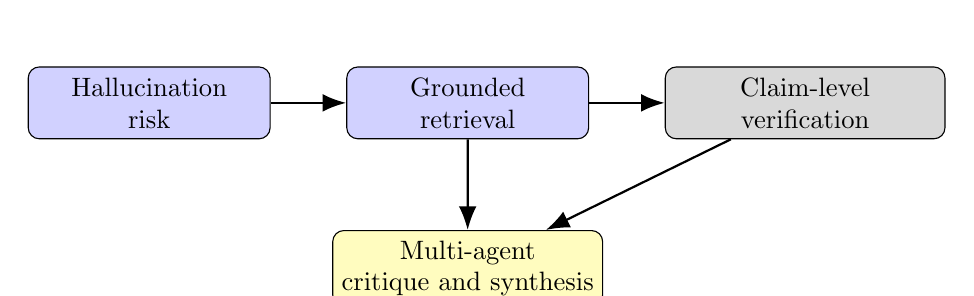
\begin{tikzpicture}[
    scale=0.96,
    transform shape,
    node distance=1.2cm and 1.0cm,
    box/.style={rectangle, rounded corners, draw=black, align=center, minimum width=3.2cm, minimum height=0.95cm, fill=blue!18},
    claim/.style={rectangle, rounded corners, draw=black, align=center, minimum width=3.7cm, minimum height=0.95cm, fill=gray!30},
    synth/.style={rectangle, rounded corners, draw=black, align=center, minimum width=3.4cm, minimum height=1.0cm, fill=yellow!25},
    arrow/.style={-{Latex[length=3mm]}, thick}
]
\node[box] (a) {Hallucination\\risk};
\node[box, right=of a] (b) {Grounded\\retrieval};
\node[claim, right=of b] (c) {Claim-level\\verification};
\node[synth, below=of b] (d) {Multi-agent\\critique and synthesis};
\draw[arrow] (a) -- (b);
\draw[arrow] (b) -- (c);
\draw[arrow] (c) -- (d);
\draw[arrow] (b) -- (d);
\end{tikzpicture}
\caption{Literature-to-design mapping for AI-Scientist}
\label{fig:lit_to_design}
\end{figure}

\section{Hallucination, Grounding, and Retrieval}

The first major theme in the literature is hallucination. In the context of scientific question answering, hallucination refers to fluent but unsupported output: a model may present a claim confidently even when the evidence does not justify it. This is especially problematic in research settings because incorrect claims can distort interpretation, misrepresent prior work, or create the impression of certainty where the literature is actually mixed \cite{manakul2023selfcheckgpt,min2023factscore,ji2023hallucination}. The literature therefore strongly supports the idea that trustworthy systems must expose their evidence rather than hiding it.

Retrieval-augmented generation addresses this issue by connecting a model to external text \cite{lewis2020rag,guu2020realm}. Instead of relying only on internal memory, the system fetches documents or passages that are relevant to the question and conditions the answer on those passages. This improves groundedness and gives the model a stronger factual basis. The key lesson for AI-Scientist is that retrieval is necessary, while effective verification still depends on interpretation, comparison, and support checking.

That observation is important because scientific tasks are rarely solved by quoting one passage. A real answer may depend on multiple papers, overlapping claims, and subtle differences in experimental setup. For that reason, the thesis treats retrieval as the first step in a wider verification pipeline rather than as the final answer mechanism. This framing keeps the system research-oriented and makes the later verification and critique stages more meaningful.

\begin{table}[H]
\centering
\begin{tabularx}{\linewidth}{>{\raggedright\arraybackslash}p{0.28\linewidth} >{\raggedright\arraybackslash}X}
\toprule
System idea & What it contributes to this thesis \\
\midrule
Plain generation & Produces fluent answers with limited evidence traceability \\
RAG & Adds external evidence and improves grounding \\
Retrieval + ranking & Helps choose the most relevant source passages \\
AI-Scientist & Uses retrieval as the input to claim verification, critique, and synthesis \\
\bottomrule
\end{tabularx}
\caption{How retrieval-oriented systems differ in the thesis context}
\end{table}

\section{Claim Verification and Structured Evaluation}

The second major theme is scientific claim verification \cite{thorne2018fever,wadden2020scifact,honovich2022true}. This literature is especially important because it matches the unit of analysis used by AI-Scientist. Instead of evaluating an entire answer as a single blob of text, claim verification decomposes the answer into smaller statements and checks each one against evidence. This is a stronger and more research-friendly approach because support, contradiction, and uncertainty are often mixed together in a single response.

Claim-level verification also makes evaluation easier to interpret. If one claim is supported and another is contradicted, the system can report that difference explicitly rather than hiding it in an averaged score. That is why this thesis later uses not only overall accuracy, but also claim-level precision, recall, and F1-score. These metrics are particularly useful because they capture how well the system identifies supported claims, how often it misses them, and how cleanly it separates correct from incorrect verdicts.

Another useful insight from the literature is that evidence should not only be present; it should be attributable. A verdict without evidence is not very useful in a scientific setting because the reader cannot inspect why the system chose that conclusion. The fact-checking and claim-verification literature consistently emphasizes rationales, supporting sentences, and explicit labels such as supported, contradicted, or insufficient evidence \cite{wadden2020scifact,thorne2018fever,min2023factscore}. AI-Scientist adopts the same idea and applies it in an orchestrated setting.

\section{Self-Critique, Multi-Agent Reasoning, and Orchestration}

The third major theme is self-critique and multi-step reasoning. Single-pass generation is fast, but it often benefits from an additional layer of review when research-grade support is required. The literature shows that systems improve when they are allowed to revise their own outputs, ask follow-up questions, or re-examine weak statements before finalizing an answer \cite{shinn2023reflexion,asai2024selfrag,yao2023treeofthoughts}. This thesis follows that idea in a structured way, using a dedicated critic stage to make the reasoning process more disciplined and inspectable.

Multi-agent orchestration is the natural way to organize that process \cite{wu2023autogen,li2023camel,du2023debate}. A retrieval agent can focus on finding evidence, a claim-extraction agent can break the evidence into checkable statements, a verification agent can decide whether the statements are supported, and a critic agent can re-check weak or contradictory claims. Finally, a synthesis agent can assemble a coherent response. This separation of responsibilities is valuable because it makes the reasoning process clearer and the system behavior easier to analyze.

The important point from the literature is that multiple agents become especially valuable when their roles are specialized. When each agent has a focused purpose, the full pipeline becomes more disciplined and more inspectable. That makes the thesis stronger because the architecture is presented as a deliberate verification workflow with clear research value.

\begin{figure}[H]
\centering
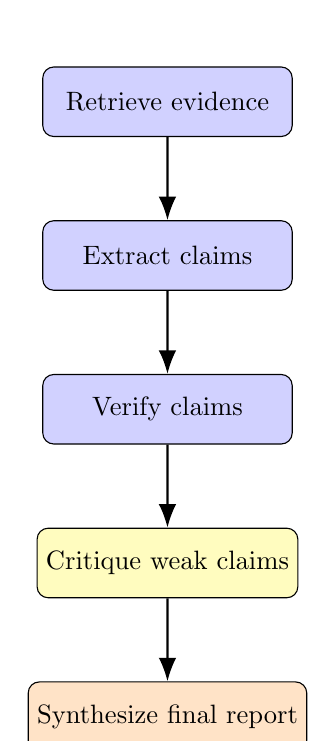
\begin{tikzpicture}[
    scale=0.96,
    transform shape,
    node distance=1.1cm,
    box/.style={rectangle, rounded corners, draw=black, align=center, minimum width=3.3cm, minimum height=0.92cm, fill=blue!18},
    critique/.style={rectangle, rounded corners, draw=black, align=center, minimum width=3.3cm, minimum height=0.92cm, fill=yellow!25},
    synth/.style={rectangle, rounded corners, draw=black, align=center, minimum width=3.3cm, minimum height=0.92cm, fill=orange!22},
    arrow/.style={-{Latex[length=3mm]}, thick}
]
\node[box] (r) {Retrieve evidence};
\node[box, below=of r] (e) {Extract claims};
\node[box, below=of e] (v) {Verify claims};
\node[critique, below=of v] (c) {Critique weak claims};
\node[synth, below=of c] (s) {Synthesize final report};
\draw[arrow] (r) -- (e);
\draw[arrow] (e) -- (v);
\draw[arrow] (v) -- (c);
\draw[arrow] (c) -- (s);
\end{tikzpicture}
\caption{Conceptual multi-agent workflow reflected in AI-Scientist}
\label{fig:multi_agent_workflow}
\end{figure}

\section{Implications for the Thesis Design}

The literature reviewed above leads to several practical implications for AI-Scientist. First, grounding should be visible, not hidden. Second, verification should happen at the claim level, not only at the answer level. Third, critique should be a deliberate stage in the pipeline so that weak conclusions can be revisited before final reporting. Fourth, confidence should be explicit because it helps the user understand which conclusions are strongly supported and which are merely plausible \cite{kadavath2022language,lin2021truthfulqa}. Finally, the complete pipeline should be traceable so that the reasoning can be explained in a thesis, defended in a viva, and inspected by another researcher.

These implications shape the structure of the remaining chapters. The architecture chapter will show how the agents are connected. The implementation chapter will explain how each agent behaves. The evaluation chapter will then test whether the framework produces strong results on the benchmark and whether the critic loop improves the outcome.

\section{Comparison of Themes}

Table~\ref{tab:related_work_comparison} provides a compact comparison of the literature themes and their relevance to the thesis.

\begin{table}[H]
\centering
\begin{tabularx}{\linewidth}{>{\raggedright\arraybackslash}p{0.22\linewidth} >{\raggedright\arraybackslash}p{0.23\linewidth} >{\raggedright\arraybackslash}X}
\toprule
Theme & Main strength & Thesis relevance \\
\midrule
Hallucination studies & Identify failure modes in model output & Justify the need for evidence grounding \\
RAG & Bring external evidence into generation & Provide the retrieval backbone \\
Claim verification & Judge claims against evidence & Enable claim-level verdicts and metrics \\
Self-critique & Revise weak outputs through feedback & Support re-verification of uncertain claims \\
Multi-agent orchestration & Separate responsibilities across stages & Make the full workflow transparent \\
\bottomrule
\end{tabularx}
\caption{Comparison of related-work themes}
\label{tab:related_work_comparison}
\end{table}

\section{Chapter Summary}

This chapter showed that AI-Scientist is grounded in a strong and coherent research tradition. The literature supports the need for grounded retrieval, claim-level verification, explicit confidence, and structured critique. It also shows why a multi-agent architecture is a natural fit for the problem: the system needs to separate evidence finding, claim checking, critique, and synthesis into distinct stages. The next chapter formalizes the problem statement and explains the requirements of the proposed framework in more detail.


\chapter[Problem Statement]{Problem Statement, Requirements, and Scope}\label{chapter:problem_statement}

\ChapterOpeningNote{This chapter formalizes the AI-Scientist task, defines the verdict space and the layered
evidence model, states the verification and honesty requirements, and fixes the practical scope of the thesis so
later architecture and evaluation claims remain precise and defensible.}

\section{Introduction}

The previous chapter positioned AI-Scientist within the literature on grounded generation, claim verification, self-critique, and multi-agent orchestration \cite{lewis2020rag,thorne2018fever,shinn2023reflexion,wu2023autogen}. This chapter converts that background into a precise problem definition. The aim is to define the system in a way that is both technically useful and thesis-ready: every important concept should be measurable, every verdict should be interpretable, and every design choice should follow naturally from the research problem.

AI-Scientist is defined here as a verification-oriented research system that receives a scientific question, retrieves layered evidence, decomposes that evidence into checkable claims, assigns a verdict and confidence to each claim, and produces a traceable report \cite{petroni2020kilt,thakur2021beir,es2023ragas}. That framing makes the thesis stronger because it turns a broad idea into a well-scoped and academically defensible system contribution.

\begin{figure}[H]
\centering
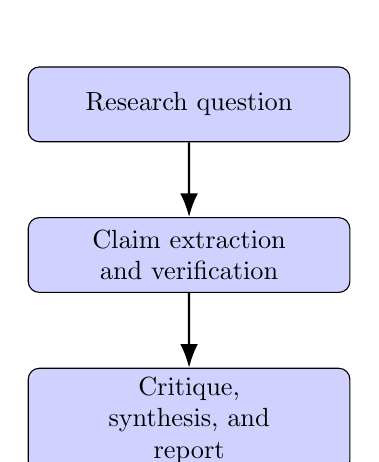
\begin{tikzpicture}[
    node distance=1.0cm,
    scale=0.95,
    transform shape,
    box/.style={rectangle, rounded corners, draw=black, fill=blue!18, align=center, minimum width=4.3cm, minimum height=1.0cm},
    arrow/.style={-{Latex[length=3mm]}, thick}
]
\node[box] (q) {Research question};
\node[box, below=of q] (r) {Claim extraction\\and verification};
\node[box, below=of r] (c) {Critique,\\synthesis, and\\report};
\draw[arrow] (q) -- (r);
\draw[arrow] (r) -- (c);
\end{tikzpicture}
\caption{Problem-definition pipeline for AI-Scientist}
\label{fig:problem_definition_pipeline}
\end{figure}

\section{Task Definition}

The task addressed in this thesis is the following: given a natural-language research question \(q\), produce a structured and grounded response using a multi-layer evidence environment \cite{guu2020realm,karpukhin2020dpr,khattab2020colbert}. The evidence environment may include user-uploaded papers, a curated offline corpus, and live scholarly sources when available. The output is a structured verification report that reflects how strongly each claim is supported by evidence, together with a concise answer that the user can read immediately after the verified claims.

This task is intentionally broader than a single retrieval setting and narrower than unrestricted generation. It is broad because it must work across domains and question types. It is focused because the system is constrained to research-oriented queries and to evidence-based verdicts. That balance makes the problem realistic and academically defensible, and it is consistent with the design direction seen in retrieval-augmented and knowledge-intensive language systems \cite{lewis2020rag,petroni2020kilt,borgeaud2022retro}.

The system input and output can be summarized as follows, following the same kind of structured specification used in benchmark-style QA and verification tasks \cite{rajpurkar2016squad,joshi2017triviaqa,yang2018hotpotqa}:
\begin{table}[H]
\centering
\begin{tabularx}{\linewidth}{>{\raggedright\arraybackslash}p{0.24\linewidth} >{\raggedright\arraybackslash}X}
\toprule
Element & Description \\
\midrule
Input question & A natural-language scientific or technical question submitted by the user \\
User evidence & Optional uploaded papers for the current session \\
Offline corpus & Curated papers that are always available for grounding \\
Live sources & Optional retrieval from scholarly APIs for broader coverage \\
Output & A structured report with claim verdicts, confidence, evidence snippets, and rationale \\
\bottomrule
\end{tabularx}
\caption{Input and output specification for AI-Scientist}
\end{table}

\begin{table}[H]
\centering
\begin{tabularx}{\linewidth}{>{\raggedright\arraybackslash}p{0.23\linewidth} >{\raggedright\arraybackslash}X}
\toprule
Verdict & Interpretation \\
\midrule
Supported & The evidence clearly aligns with the claim and provides a stable basis for the response \\
Contradicted & The evidence points in the opposite direction or introduces a direct conflict \\
Insufficient evidence & The available material is promising but not yet strong enough to justify a firm claim \\
Out of scope & The input falls outside the research-focused operating range of the system \\
\bottomrule
\end{tabularx}
\caption{Verdict interpretation used in the thesis}
\end{table}

\section{Verdict Space and Claim-Level Reasoning}

A central decision in the thesis is to make the claim, not the whole answer, the unit of reasoning \cite{honovich2022true,min2023factscore}. This is a better fit for scientific work because papers rarely support every detail of an answer equally. Some parts may be strongly supported, some may be weakly supported, and some may remain unresolved. A single answer-level label would hide these differences, whereas a claim-level verdict makes them visible and useful.

AI-Scientist therefore uses a bounded verdict space:
\begin{itemize}[leftmargin=*]
    \item \textbf{Supported} when the retrieved evidence clearly aligns with the claim,
    \item \textbf{Contradicted} when the evidence supports the opposite direction or clearly conflicts with the claim,
    \item \textbf{Insufficient evidence} when the available evidence is too weak to decide confidently,
    \item \textbf{Out of scope} when the input is not a research question and should be declined early.
\end{itemize}

This verdict space has an important thesis value: it encourages clarity without reducing the utility of the system. In other words, the system remains effective when it chooses a careful verdict. That is a strong research property because it shows that the framework knows not only how to answer, but also how to calibrate the strength of its response to the underlying evidence.

\section{Evidence Model and Relevance}

The quality of a verdict depends on the quality of evidence behind it. For this reason, AI-Scientist uses a layered evidence model rather than a flat corpus. The evidence layers are ordered by practical trust and relevance:
\begin{enumerate}[leftmargin=*]
    \item user-uploaded papers supplied for the session,
    \item curated offline corpus papers,
    \item live scholarly sources retrieved during execution.
\end{enumerate}

This structure is useful because it mirrors the way a careful researcher works. User-provided material should be respected when it is relevant, the curated corpus provides a dependable grounding baseline, and live retrieval broadens the context when extra support is needed. Source priority is therefore not a side detail; it is part of the problem definition itself, and it follows the same practical layering logic used in retrieval-oriented pipelines \cite{ragsurvey2024,es2023ragas}.

To make evidence selection transparent, the thesis uses a coverage-based relevance measure for papers and a token-overlap measure for finer sentence-level support. A paper is considered admissible when it clears a minimum relevance threshold, which helps maintain a focused and reliable verification chain while keeping the retrieval stage efficient.

\begin{equation}
\mathrm{cov}(q, d) = \frac{|T(q) \cap T(d)|}{|T(q)|}
\end{equation}

Here, \(T(q)\) and \(T(d)\) are the normalized token sets of the query and document. This formulation is attractive because it rewards a document for covering the query terms without unfairly penalizing longer abstracts. In practice, it gives the pipeline a concise first indicator of whether a paper is worth deeper inspection.

\section{Confidence and Traceability}

Confidence is treated as a first-class output in this thesis \cite{kadavath2022language,lin2021truthfulqa}. That choice is important because a scientific assistant should not only say what it believes; it should also indicate how strongly the evidence supports that belief. The confidence score combines evidence overlap, corroboration, and independence of sources. A stronger score means that multiple pieces of evidence point in the same direction and that the claim is supported by a stable evidentiary pattern rather than by a single isolated source alone.

\begin{equation}
c = \mathrm{clip}\Big(\beta_0 + \beta_1\,\mathrm{ovl}_{\max} + \beta_2\,n_{\mathrm{extra}}
+ \beta_3\,n_{\mathrm{indep}} - \gamma\,\mathbb{1}[\text{self-only}],\; c_{\min},\; c_{\max}\Big)
\end{equation}

The exact coefficients are implementation-dependent, but the thesis-level interpretation is clear: confidence should reflect the strength and breadth of evidence. This is a valuable design choice because it gives the user a compact yet meaningful signal about trust, especially when several candidate claims look plausible at first glance.

Traceability is equally important. Every verdict should retain the supporting snippets and the rationale used to reach it. That way, a reader can inspect the evidence behind a conclusion and understand why the system made a particular decision. This is especially useful in a thesis context because it makes the system easier to explain in a viva and easier to compare with alternative approaches.

\section{Scope and Non-Goals}

AI-Scientist is designed as a domain-general research assistant rather than a narrow subject-specific tool. The framework is meant to accept questions from multiple academic fields, and the verification pipeline remains consistent across domains. This is a strong design advantage because it shows that the method is not tied to one particular benchmark topic \cite{petroni2020kilt,thakur2021beir,gu2021pubmedbert}.

At the same time, the system is not intended to behave like a general-purpose chatbot. A scope guard prevents non-research queries from entering the verification pipeline. This keeps the system focused on the class of problems it is designed to solve and preserves the clarity of the thesis contribution.

The thesis also excludes several tempting but unnecessary claims:
\begin{itemize}[leftmargin=*]
    \item autonomous scientific discovery is not claimed,
    \item exhaustive literature coverage is not claimed,
    \item full-text deep reading of every paper is not required,
    \item and replacing human judgement is not the objective.
\end{itemize}

These non-goals strengthen the work because they keep the system well-scoped in a positive way: the framework is ambitious enough to be meaningful, but focused enough to be credible.

\section{Verification Requirements}

The problem definition imposes several operational requirements on the system:
\begin{itemize}[leftmargin=*]
    \item a claim may be marked supported only when evidence clearly aligns with it,
    \item contradiction must be reported explicitly when evidence conflicts,
    \item weak claims should produce insufficient evidence rather than overconfident conclusions,
    \item confidence must account for evidence strength and corroboration,
    \item and every verdict must remain traceable to its source snippets.
\end{itemize}

These requirements are the foundation of the thesis evaluation. They also explain why a claim-level metric suite is needed later on. A system that performs well under these requirements is doing more than generating text; it is performing disciplined scientific verification.

\section{Adaptive Reasoning}

One of the most valuable features of the thesis problem definition is adaptive reasoning. If a claim appears weak on the first pass, the system should be able to request more evidence and re-check the claim before finalizing the report. This makes AI-Scientist feel more like a careful researcher and less like a fixed one-shot summarizer.

The adaptive loop is deliberately bounded. It is meant to improve weak or uncertain claims, not to search indefinitely. That constraint keeps the system efficient while still allowing it to handle difficult claims in a principled way.

\begin{figure}[H]
\centering
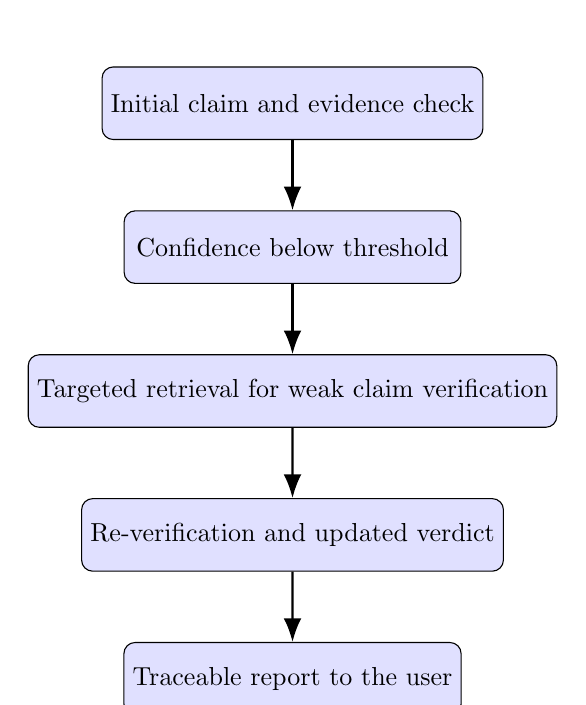
\begin{tikzpicture}[
    node distance=0.95cm,
    scale=0.94,
    transform shape,
    box/.style={rectangle, rounded corners, draw=black, fill=blue!12, align=center, minimum width=4.55cm, minimum height=0.98cm},
    arrow/.style={-{Latex[length=3mm]}, thick}
]
\node[box] (a) {Initial claim and evidence check};
\node[box, below=of a] (b) {Confidence below threshold};
\node[box, below=of b] (c) {Targeted retrieval for weak claim verification};
\node[box, below=of c] (d) {Re-verification and updated verdict};
\node[box, below=of d] (e) {Traceable report to the user};
\draw[arrow] (a) -- (b);
\draw[arrow] (b) -- (c);
\draw[arrow] (c) -- (d);
\draw[arrow] (d) -- (e);
\end{tikzpicture}
\caption{Adaptive reasoning loop used to refine uncertain claims}
\label{fig:adaptive_reasoning_loop}
\end{figure}

\section{Chapter Summary}

This chapter formalized the AI-Scientist problem as a verification-first research task. It defined the task input and output, the verdict space, the layered evidence model, confidence and traceability requirements, scope boundaries, and the adaptive reasoning loop. These definitions give the later architecture and evaluation chapters a clear foundation. The next chapter uses these requirements to describe the system architecture in detail.


\chapter[System Design]{System Design and Architecture}\label{chapter:system_design}

\ChapterOpeningNote{This chapter presents the AI-Scientist architecture, explains the role of the Orchestrator
and each specialized agent in the verification pipeline, and describes the layered evidence model and the
critic-driven re-verification loop that together realize evidence-grounded, traceable reasoning.}

\section{Introduction }

The previous chapter defined AI-Scientist as a verification-first, evidence-grounded research assistant. This
chapter shows how that definition is realized architecturally. The most important high-level point is that
AI-Scientist is not a single prompt or an unstructured collection of agents \cite{wu2023autogen,li2023camel,du2023debate}. It is a structured pipeline of
specialized agents coordinated by an explicit Orchestrator, in which control flow is deterministic and only
specific stages delegate to a language model. This design keeps the system focused, inspectable, and well suited
to thesis-level evaluation.

The architecture follows the evidence discussed in the literature review. Grounded reasoning systems are easier to
defend, inspect, and reason about when their stages and transitions are visible. AI-Scientist therefore separates
retrieval, claim extraction, verification, critique, synthesis, and reporting into distinct agents with typed
inputs and outputs. This separation gives the thesis a clear systems story: trustworthy scientific answering is not
a monolithic generation step, but a controlled workflow that transforms a research question into an
evidence-backed, confidence-annotated report.

\section{Architectural Philosophy }

AI-Scientist is best understood as a \emph{multi-agent orchestrated pipeline} with an embedded re-verification
loop \cite{yao2023treeofthoughts,shinn2023reflexion,asai2024selfrag}. A single Orchestrator owns the workflow state and invokes each agent in turn; the agents do not coordinate
autonomously among themselves. In the terminology used throughout the project:

\begin{enumerate}
\item an \textbf{agent} is a component with one specialized responsibility (retrieval, extraction, verification,
critique, synthesis, or reporting);
\item a \textbf{deterministic stage} uses fixed rules, token-overlap measures, and thresholds and does not call a
language model;
\item an \textbf{LLM-backed stage} performs bounded model-assisted refinement on top of a deterministic result;
and
\item the \textbf{critic loop} is the adaptive act-observe-revise step in which the Critic's assessment of weak
claims feeds a second, targeted retrieval-and-verification pass.
\end{enumerate}

This distinction matters because it clarifies where each capability contributes most effectively. The backbone of
AI-Scientist --- retrieval ranking, evidence scoring, verdict selection, confidence computation, and critique ---
is deterministic and therefore reproducible and inspectable. Language-model assistance is layered on selected
stages as an optional refinement, and the system degrades gracefully to its deterministic behaviour when no model
is available. This separation mirrors the direction of agentic and retrieval-augmented systems that favor explicit control surfaces over a single opaque generation step \cite{lewis2020rag,guu2020realm,langgraph2024}.
Figure~\ref{fig:architecture} shows the high-level organization, and Figure~\ref{fig:pipeline} shows the
end-to-end data flow including the critic loop.

The overall division of responsibilities is summarized in Table~\ref{tab:agent_roles}.

\begin{table}[!htbp]
\centering
\caption{Specialized agents and their primary responsibilities}
\label{tab:agent_roles}
\begin{tabularx}{\linewidth}{>{\raggedright\arraybackslash}p{0.25\linewidth} >{\raggedright\arraybackslash}X}
\toprule
Agent & Primary responsibility \\
\midrule
Orchestrator & Coordinates workflow state, scope control, and stage transitions \\
Retrieval & Finds and ranks evidence from uploads, corpus, and live sources \\
Claim Extraction & Converts evidence into checkable scientific claims \\
Verification & Assigns verdicts and confidence using evidence support \\
Critic & Identifies weak claims and triggers targeted re-verification \\
Synthesis & Produces the concise final answer from verified claims \\
Report & Assembles the traceable structured output for the user \\
\bottomrule
\end{tabularx}
\end{table}

\begin{figure}[!htbp]
\centering
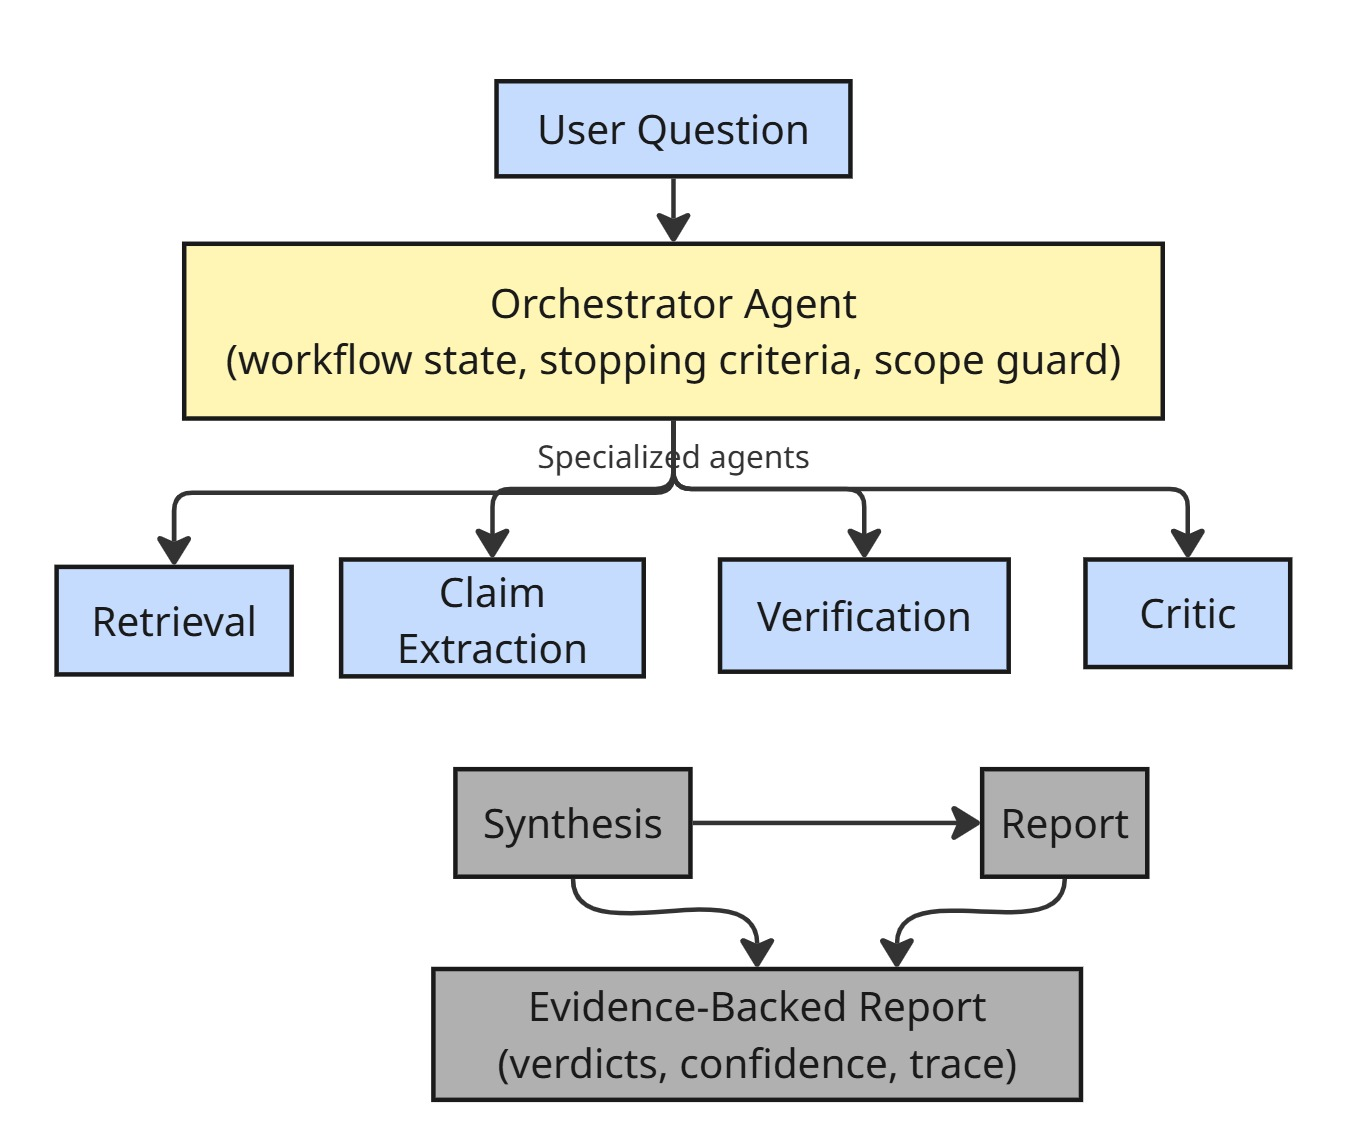
\includegraphics[draft=false,width=0.72\linewidth]{Fig_4.1.jpg}
\caption[High-level AI-Scientist architecture]{\textbf{High-level AI-Scientist architecture.} A single
Orchestrator coordinates the specialized agents and produces an evidence-backed report with verdicts,
confidence, and traceability.}
\label{fig:layered_system_view}
\label{fig:architecture}
\end{figure}

\section{The Orchestrator Agent }

The Orchestrator is the central controller of AI-Scientist. It receives the user's research question, applies the
scope guard, and then drives the agents in a fixed order: retrieve evidence, extract claims, verify each claim,
criticize the results, optionally re-verify weak claims, synthesize a summary, and build the report \cite{langgraph2024,wu2023autogen}.
It also owns
the workflow's early-exit conditions: if the question is out of scope, if no relevant papers are found, or if no
sufficiently aligned claims can be extracted, the Orchestrator stops early and returns an honest report explaining
why, rather than forcing the pipeline forward into an uncertain conclusion.

Crucially, the Orchestrator maintains the \emph{orchestration trace} --- a running list of human-readable steps
describing what happened at each stage, such as how many papers were retrieved, how many claims were extracted,
how many critique notes were raised, and whether a second verification pass was triggered. This trace is part of
the final report and is the mechanism by which the system's reasoning becomes inspectable.

This trace also creates a convenient thesis artifact. It turns the internal workflow into a visible sequence that
can be discussed in text, displayed in the interface, and examined during evaluation. In that sense, the
Orchestrator is not just a control component; it is the layer that makes the entire pipeline legible to the user.

\section{The Evidence Layer and the Retrieval Agent }

The Retrieval agent realizes the layered evidence model from Chapter~3. It maintains a local pool that lists
user-uploaded papers first and then the curated corpus, deduplicated so that an uploaded paper wins on a tie. When
live retrieval is enabled, it augments this local pool with results fetched at query time from PubMed Central and
arXiv \cite{lewis2020rag,guu2020realm,karpukhin2020dpr,khattab2020colbert}.

Ranking is where the source-priority requirement becomes concrete. Each candidate paper is scored by its
query-coverage relevance plus a source-dependent bonus, with uploaded papers receiving the largest bonus, curated
corpus papers an intermediate bonus, and live-API papers the smallest. Candidates are then admitted only if their
raw coverage clears the minimum threshold, so the source bonus changes ordering but cannot smuggle in an
irrelevant paper. The agent also applies a quality filter to live results --- penalizing very short or metadata-poor
abstracts --- so that low-quality API hits do not dilute the evidence pool. The result is a ranked evidence set in
which user-provided and locally trusted papers surface first, while genuinely relevant live results can still
appear.

This ranking logic is important because it gives the architecture a practical notion of evidence preference. It
allows the system to stay responsive to the user's own materials, remain grounded in a reliable offline corpus, and
still extend outward when the question benefits from broader coverage. The evidence layer therefore supports both
precision and flexibility.

\section{The Claim Extraction Agent }

Once evidence has been retrieved, the Claim Extraction agent converts the unstructured abstracts into discrete,
checkable claims \cite{thorne2018fever,wadden2020scifact}. It scans each retrieved paper sentence by sentence and selects candidate statements that either
contain research-assertion cues (such as ``improves,'' ``reduces,'' ``demonstrates,'' or ``outperforms'') or share
content tokens with the user's question. Each selected sentence becomes a structured claim that records its text, a
coarse claim type (performance, finding, implication, limitation, or observation), its source paper, and the focus
terms it shares with the question.

This stage is the architectural embodiment of the claim-level factuality principle from the literature. By turning
a paper into a small set of explicit claims, AI-Scientist ensures that verification, confidence, and critique all
operate at the granularity where support and contradiction actually differ, rather than on a single fused answer.
The number of claims per question is bounded so that the workflow stays focused on the statements most relevant to
the query.

This bounded extraction stage has two practical benefits. First, it keeps the downstream verifier focused on the
claims that matter most for the question. Second, it gives the thesis a clean object of analysis: each extracted
statement can be tracked, scored, and discussed individually. That makes the system easier to evaluate and the
writing easier to defend.

\section{The Verification Agent }

The Verification agent is the analytical core of AI-Scientist. For each claim, it examines the sentences of the
candidate papers and computes an evidence score that blends Jaccard overlap with focus-term and content-term
agreement, plus small bonuses when a sentence comes from the claim's own source or matches its rhetorical type. It
then classifies each scored sentence as supporting or contradicting the claim, using negation and
contradiction-cue analysis: a sentence whose polarity disagrees with the claim's polarity is treated as
contradictory.

From the collected evidence, the agent selects one of the four verdicts defined in Chapter~3. A claim with
adequate aligned support becomes supported; a claim where strong, multi-source counter-evidence dominates becomes
contradicted; an overgeneralized claim, or one without sufficient overlap, becomes insufficient evidence. The
confidence attached to each verdict is computed deterministically from evidence strength, the number of additional
supporting snippets, and the number of independent corroborating sources, with an explicit penalty when a claim is
only self-corroborated. This is the architectural point at which the honesty requirements become operational:
verdicts are bound to evidence, contradictions are representable, and self-corroboration is discounted.

The deterministic confidence computation is valuable from a thesis perspective because it produces a stable and
interpretable signal. The score is not arbitrary; it reflects observable evidence properties that can be explained
clearly in text, compared across claims, and discussed during evaluation.

When a language model is available, the verifier can pass its preliminary verdict, together with the selected
supporting and contradicting snippets, to a bounded refinement step that may adjust the verdict and rationale. This
refinement is constrained to the already-retrieved evidence and is optional; if it is unavailable or fails, the
deterministic assessment stands.

\section{The Critic Agent and the Re-Verification Loop }

The Critic agent implements the adaptive-reasoning requirement \cite{shinn2023reflexion,yao2023treeofthoughts,asai2024selfrag}. After the first verification pass, it reviews all
assessments and raises critique notes for four weakness patterns: claims with insufficient evidence, claims whose
confidence falls below a threshold, claims supported by only a single source, and claims that are contradicted.
These notes are reported to the user, but more importantly they can drive action.

For claims that are weak in a way that more evidence might resolve, the Critic produces a re-verification decision:
a targeted follow-up query built from the claim text, its focus terms, and its source title, with an added
counter-evidence probe when the claim contains absolute or contradiction-prone language. The Orchestrator then
runs a second retrieval pass for that specific claim, merges the new papers with the first-pass evidence, and
re-verifies the claim with a preference for resolving contradictions. Overgeneralized claims are deliberately
excluded from this loop, because seeking more evidence cannot rescue a claim that is too broad to settle.

This loop is the architectural difference between AI-Scientist and a fixed RAG pipeline \cite{lewis2020rag,ragsurvey2024}. The effort spent on a
claim is conditioned on how uncertain the first pass was, and the additional retrieval is aimed precisely at the
weak claim rather than re-running the whole query. Figure~\ref{fig:pipeline} shows this feedback path explicitly.

The loop is also thesis-friendly because it demonstrates controlled adaptivity. The system responds to weak
evidence by deciding where additional effort should be spent. That makes the design feel deliberate and
research-oriented.

\begin{figure}[!htbp]
\centering
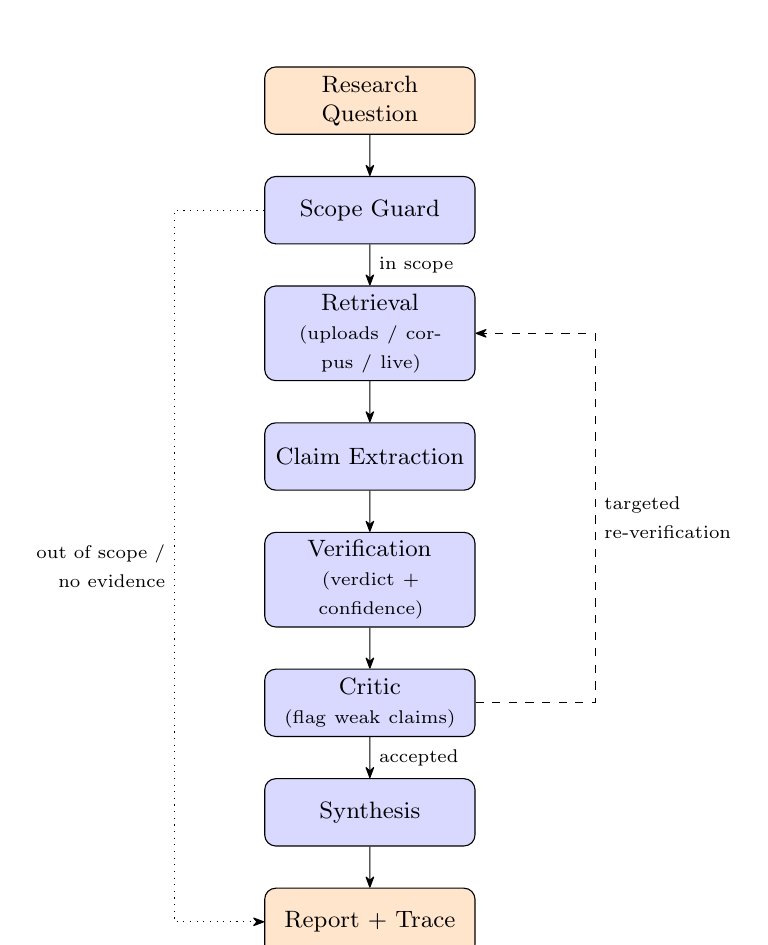
\begin{tikzpicture}[
  font=\small,
  node distance=5.5mm,
  scale=0.95,
  transform shape,
  stage/.style={draw, rounded corners, align=center, text width=26mm, minimum height=9mm, inner sep=3pt, fill=blue!15},
  io/.style={draw, rounded corners, align=center, text width=26mm, minimum height=9mm, inner sep=3pt, fill=orange!20},
  >={Stealth[round]}
]
\node[io] (q) {Research Question};
\node[stage, below=of q] (scope) {Scope Guard};
\node[stage, below=of scope] (ret) {Retrieval\\ \scriptsize (uploads / corpus / live)};
\node[stage, below=of ret] (claim) {Claim Extraction};
\node[stage, below=of claim] (ver) {Verification\\ \scriptsize (verdict + confidence)};
\node[stage, below=of ver] (crit) {Critic\\ \scriptsize (flag weak claims)};
\node[stage, below=of crit] (syn) {Synthesis};
\node[io, below=of syn] (rep) {Report + Trace};

\draw[->] (q) -- (scope);
\draw[->] (scope) -- (ret) node[midway,right]{\scriptsize in scope};
\draw[->] (ret) -- (claim);
\draw[->] (claim) -- (ver);
\draw[->] (ver) -- (crit);
\draw[->] (crit) -- (syn) node[midway,right]{\scriptsize accepted};
\draw[->] (syn) -- (rep);

% critic re-verification loop
\draw[->, dashed] (crit.east) -- ++(16mm,0) |- (ret.east)
  node[pos=0.25, right, align=left]{\scriptsize targeted\\ \scriptsize re-verification};

% early exits
\draw[->, dotted] (scope.west) -- ++(-12mm,0) |- (rep.west)
  node[pos=0.25, left, align=right]{\scriptsize out of scope /\\ \scriptsize no evidence};
\end{tikzpicture}
\caption[The AI-Scientist verification pipeline]{\textbf{The AI-Scientist verification pipeline end-to-end.} A
research question passes the scope guard, is grounded by layered retrieval, decomposed into claims, and verified
into per-claim verdicts with confidence. The Critic flags weak claims and can trigger a targeted re-verification
pass (dashed). Honest early exits (dotted) return a report when the question is out of scope or no relevant
evidence exists. Synthesis and reporting produce the final evidence-backed report and orchestration trace.}
\label{fig:pipeline}
\end{figure}

\section{The Synthesis Agent }

The Synthesis agent composes the executive summary from the verified claims and the critique notes. Its
deterministic form aggregates the assessments into a short, calibrated statement: how many claims are supported,
how many are contradicted, and how many remain unresolved, with an explicit note that weakly supported or
contradicted claims should be read cautiously. When a language model is available, the agent can rewrite this
summary into more fluent prose under tight constraints --- it is instructed to state the overall finding in a few
sentences, to remain grounded in the verified claims, and not to overclaim --- and it falls back to the
deterministic summary if the model is unavailable.

The architectural significance of this stage is that synthesis is downstream of verification, not a substitute for
it. The summary describes the verified evidence and does not introduce new conclusions that were not checked.

This stage directly supports the user-facing answer that appears in the interface. It bridges the gap between
claim-by-claim verification and a concise conclusion, so the final report remains readable without losing its
evidence trail. In thesis terms, it shows how a structured system can be both rigorous and approachable.

\section{The Report Agent and the Orchestration Trace }

The Report agent assembles the final structured output: the question, the executive summary, the list of retrieved
papers, the orchestration trace, the per-claim verification details (claim text, type, source, verdict, confidence,
rationale, and evidence snippets), and the critique notes. The report is produced as both a structured object and a
rendered Markdown document so that it can be displayed in the user interface, returned through the API, or exported.

The trace-based design is intentional. Because the thesis emphasizes trustworthy reasoning, the system should
output more than a conclusion. The conclusion must be inspectable, explainable, and attributable to its
intermediate stages. A reader can see why a claim was marked insufficient, which paper supported a supported claim,
and whether a second verification pass was run.

This reporting format also makes the system practical for real use. A researcher can read the final answer quickly,
inspect the verified claims when needed, and use the trace to understand how the system reached its position.
That combination of brevity and accountability is especially valuable in an academic setting.

\section{Graceful Degradation and the Optional LLM Layer }

A defining architectural property of AI-Scientist is that the language model is an optional accelerator rather than
a hard dependency. The Verification and Synthesis agents consult a provider-backed model only when one is
configured; otherwise the system runs entirely on its deterministic heuristics. The model layer is also written to
tolerate provider differences: reasoning-capable models receive an effort parameter, while chat models that reject
that parameter are detected and called without it, and any model failure is logged and falls back to the
deterministic result.

This design serves three purposes. First, it makes the core pipeline reproducible and offline-capable, which is
essential for a thesis that emphasizes inspectable reasoning rather than opaque cloud orchestration. Second, it
lets the model improve fluency and borderline verdicts without ever being able to override the grounding and
honesty rules, because those rules run first and constrain what the model sees. Third, it keeps the architecture
model-agnostic, so the system is not tied to a single vendor.

In practice, this makes the system attractive for both demonstration and research. The deterministic core provides
reliability, while the optional language-model layer adds fluency and polish where appropriate. The result is a
balanced design that remains stable even when external services are unavailable.

\section{Why the Architecture Matches the Thesis Claim }

The AI-Scientist architecture is a direct structural expression of the thesis claim rather than a simple sequence
of implementation modules. The system begins by grounding reasoning in layered, source-prioritized evidence
rather than trusting the model's parametric memory, decomposes that evidence into discrete claims, verifies each
claim against evidence with explicit confidence, criticizes the weak claims and re-verifies them adaptively, and
records a trace of the whole process. In doing so, it embodies four commitments:

\begin{enumerate}
\item \textbf{Evidence grounding:} reasoning is bound to retrieved sources, not to generation.
\item \textbf{Calibrated confidence:} every verdict carries a transparent confidence derived from evidence
strength, corroboration, and independence.
\item \textbf{Self-critique:} a separate Critic agent flags weak claims and can demand more evidence.
\item \textbf{Traceability:} the orchestration trace and per-claim evidence make every conclusion auditable.
\end{enumerate}

These commitments distinguish AI-Scientist from both single-pass readers and standard RAG pipelines while keeping
the design compact and academically coherent.

They also explain why the architecture is well matched to the thesis goal. Each major design choice maps to a
research concern: grounding, confidence calibration, critique, or traceability. That alignment makes the chapter a
natural bridge between the problem definition and the implementation details that follow.

\section{Chapter Conclusion }

This chapter described the AI-Scientist system design as a structured, orchestrated verification pipeline rather
than a generic language-model application. The architecture begins with layered retrieval, moves through claim
extraction and deterministic evidence-bound verification, narrows uncertainty through the Critic agent and a
targeted re-verification loop, and ends with synthesis and a traceable report. The language model is an optional
refinement layer that never overrides the grounding and honesty rules. With the architecture now established, the
next chapter maps these agents to the actual implementation.



\chapter[Implementation]{Implementation}\label{chapter:implementation}

\ChapterOpeningNote{This chapter maps the AI-Scientist architecture to the codebase, showing how the
orchestrated verification pipeline is implemented in modular agent components, how grounding and confidence are
computed in practice, and how the system remains usable even when the optional language-model layer is
unavailable.}

\section{Introduction}

The previous chapter described the AI-Scientist architecture as an orchestrated verification pipeline. This chapter
maps that design onto the actual implementation. The goal is not to list every file mechanically, but to explain
how the main modules cooperate to realize evidence-grounded, self-critical, traceable verification in code.

The implementation is organized as a single Python package, \texttt{ai\_scientist}, with the agents in an
\texttt{agents} subpackage and a set of supporting modules for configuration, data models, corpus access,
ingestion, retrieval utilities, scope control, and the optional language-model layer. A Streamlit user interface
and a programmatic API sit on top of the same package. This separation is intentional: the package contains the
reasoning logic, while the interfaces are thin clients that drive it.

\section{Implementation Structure}

At the highest level, the codebase is divided into:

\begin{enumerate}
\item \textbf{agent modules} under \path{ai_scientist/agents/}, which implement retrieval, claim extraction,
verification, critique, synthesis, reporting, and live retrieval;
\item \textbf{the orchestrator} in \path{ai_scientist/agents/orchestrator.py}, which wires the agents into the
end-to-end workflow;
\item \textbf{core modules} --- \path{models.py}, \path{config.py}, \path{corpus.py}, \path{ingestion.py},
\path{utils.py}, \path{scope.py}, and \path{llm.py} --- which provide the data types, settings, evidence access,
and shared logic;
\item \textbf{baselines} in \path{baselines.py}, which implement the single-agent and RAG comparison systems on
top of the same retrieval and scoring code; and
\item \textbf{interfaces}: a Streamlit application (\path{app.py}) and a FastAPI service
(\path{ai_scientist/api.py}).
\end{enumerate}

This layered structure keeps the reasoning system reusable. The same \texttt{analyze\_question(...)} entry point
used by the user interface is also used by the API and by the baselines harness, so that what is demonstrated is
the real system rather than a simplified mock-up.

\section{Typed Data Models}

The pipeline communicates through explicit dataclasses defined in \path{models.py}. A \texttt{PaperDocument}
carries a paper's identifier, title, abstract, year, authors, and topics. A \texttt{StructuredClaim} records a
claim's text, type, source paper, source sentence, and focus terms. An \texttt{EvidenceSnippet} pairs a sentence
with its overlap score and source. A \texttt{ClaimAssessment} bundles a claim with its verdict, confidence,
evidence list, and rationale. Finally, a \texttt{FinalReport} aggregates the question, summary, verified claims,
critique notes, retrieved papers, rendered Markdown, and the iteration trace.

These typed structures are important because every stage writes to a shared, serializable interface rather than
passing unstructured text. This is what makes the system auditable: the report is not a paragraph that happens to
mention sources, but a structured object in which each conclusion is explicitly linked to its evidence.

\section{The Orchestrator}

The practical center of the implementation is \texttt{MultiAgentResearchSystem} in \path{orchestrator.py}. Its
\texttt{analyze\_question} method realizes the workflow described in Chapter~4: it applies the scope guard,
retrieves evidence, extracts claims, verifies them through a refinement routine, runs the Critic, optionally
re-verifies weak claims, synthesizes the summary, and builds the report. The method also implements the honest
early exits: if the question is out of scope, if retrieval returns no papers, or if no aligned claims can be
extracted, it returns a report that explains the situation instead of fabricating an answer.

Adaptive re-verification is implemented in the private \texttt{\_refine\_assessments} and \texttt{\_run\_second\_pass}
routines. After the first pass, the Critic's \texttt{identify\_reverification\_targets} produces a list of
follow-up decisions; for each, the Orchestrator retrieves additional papers for that claim's follow-up query,
merges them with the first-pass evidence, and re-verifies the claim with contradiction resolution preferred. Every
step appends a human-readable line to the iteration trace, which is what the user ultimately sees as the
orchestration trace.

\section{Retrieval and the Layered Evidence Pool}

The Retrieval agent in \path{agents/retrieval.py} implements the layered evidence model. Its \texttt{\_local\_pool}
builds a deduplicated pool that lists uploaded papers before curated-corpus papers, and \texttt{\_local\_rank\_score}
adds the source-dependent bonus so that uploads outrank corpus papers at comparable relevance. The
\texttt{\_rank\_subset} routine ranks candidates by this source-weighted score but gates admission on the raw
query-coverage clearing the configured minimum, so the bonus can reorder evidence but never inject an irrelevant
paper.

When live retrieval is enabled, \texttt{retrieve} layers API results on top of the local pool. Live papers pass
through a quality filter that rewards adequate abstract length, query relevance in title and abstract, recency, and
the presence of research-indicator terms, and they are merged with a strict source priority: uploads first, then
corpus, then live. A title-similarity check removes near-duplicates so the same paper is not counted twice across
sources. The agent is wrapped so that any network failure falls back cleanly to the local pool, keeping the system
usable offline.

\section{Retrieval Utilities}

The relevance measures live in \path{utils.py}. Tokenization normalizes case, strips stopwords, and applies a
small morphological normalization so that, for example, plural and singular forms of common research terms match.
On top of tokenization, \texttt{overlap\_score} computes Jaccard overlap for short-text comparison, and
\texttt{coverage\_score} computes the length-robust query coverage used for paper-level ranking. Keeping both
measures in one module makes the design decision from Chapter~3 --- coverage for ranking, Jaccard for
sentence-level evidence --- explicit and reusable across the verifier, the retriever, and the baselines.

\section{Claim Extraction}

The Claim Extraction agent in \path{agents/claim_extraction.py} scans each retrieved paper sentence by sentence. A
sentence becomes a candidate claim if it contains a positive research cue or shares content tokens with the
question. Each candidate is wrapped in a \texttt{StructuredClaim} whose type is inferred from surface cues ---
limitation, performance, finding, implication, or observation --- and whose focus terms are the intersection of the
question and sentence tokens. Extraction stops once a configured maximum number of claims is reached, keeping the
workflow focused on the statements most relevant to the query.

\section{Verification}

The Verification agent in \path{agents/verification.py} is the analytical heart of the implementation. For each
claim it iterates over the sentences of the candidate papers and computes an evidence score that combines Jaccard
overlap with focus-term and content-term agreement and small type- and source-aware bonuses. Each scored sentence
is then classified as supporting or contradicting the claim, using negation and contradiction-cue analysis so that
a polarity mismatch between claim and sentence is treated as a contradiction.

From the collected evidence the agent selects a verdict. An overgeneralized claim returns insufficient evidence
unless a contradiction pass is explicitly requested; strong, multi-source counter-evidence yields a contradicted
verdict; adequate aligned support yields a supported verdict; and the absence of sufficient overlap yields
insufficient evidence. Confidence is computed by \texttt{\_supported\_confidence} and \texttt{\_contradicted\_confidence}
from the strongest evidence overlap, the count of additional supporting snippets, and the number of independent
corroborating sources, with an explicit penalty when a claim is corroborated only by its own source. All confidence
values are clamped between a floor and a ceiling so the system never reports absolute certainty. The optional
language-model refinement is invoked only after this deterministic assessment is formed, and only over the
evidence already selected.

\section{Critique and Adaptive Re-Verification}

The Critic agent in \path{agents/critic.py} implements both reporting and adaptivity. Its \texttt{critique} method
produces notes for insufficient, low-confidence, single-source, and contradicted claims, including details such as
whether a single-source claim is merely self-corroborated. Its \texttt{identify\_reverification\_targets} method
selects which weak claims warrant another pass and builds a follow-up query from the claim text, its focus terms,
its source title, and a counter-evidence probe when the claim uses absolute or contradiction-prone language.
Overgeneralized claims are excluded, because additional retrieval cannot settle a claim that is too broad. This is
the implementation of the bounded, targeted adaptivity required in Chapter~3.

\section{Synthesis and Reporting}

The Synthesis agent in \path{agents/synthesis.py} aggregates the assessments into a calibrated summary, optionally
rewritten by the language model under instructions to stay grounded and avoid overclaiming, with a deterministic
fallback. The Report agent in \path{agents/report.py} renders the structured \texttt{FinalReport}, including the
retrieved papers, the orchestration trace, and the full per-claim verification details with evidence snippets and
overlap scores. Because the report is both a structured object and rendered Markdown, the same result can be shown
in the interface, returned by the API, or exported.

\section{The Optional Language-Model Layer}

The language-model abstraction in \path{llm.py} wraps a provider client behind a single interface. It is available
only when an API key is configured; otherwise the agents run on their deterministic logic. The module is written to
be provider-tolerant: a helper detects whether the configured model accepts a reasoning-effort parameter and
includes it only for reasoning-capable models, while models that would reject it are called without it. Structured
outputs are parsed into small typed schemas for the refined verdict and the rewritten summary, and any call failure
is logged and degrades to the deterministic result rather than breaking the pipeline.

This design serves three purposes. First, it makes the core pipeline reproducible and offline-capable. Second, it
ensures the model can improve fluency and borderline verdicts but can never bypass the grounding and honesty rules,
which run first. Third, it keeps the system model-agnostic, so a different model or provider can be substituted
through configuration.

\section{Live Scholarly Retrieval}

Live evidence is implemented in \path{agents/live_retrieval.py}. The agent queries PubMed Central through the NCBI
E-utilities (search, summary, and fetch) and arXiv through its Atom API. Two implementation details are important
for evidence quality. First, PubMed Central searches are sorted by relevance rather than date, because the default
date ordering surfaces recent but off-topic papers. Second, abstracts in the PubMed Central XML are nested inside
structured elements, so the agent gathers all descendant text rather than only the top-level text node, which is
what allows it to recover full abstracts instead of empty placeholders. The agent also derives cleaner search
variants from a natural-language question by removing generic filler words, and it identifies itself to NCBI and
backs off on rate-limit responses, optionally using an API key to raise the request rate.

\section{Configuration and Scope}

Behaviour is centralized in the \texttt{Settings} dataclass in \path{config.py}, which holds the retrieval depth,
the coverage and support thresholds, the confidence floor and ceiling, the source-priority bonuses, the model
configuration, and the keyword lists used by the scope guard. Settings can be constructed directly or built from
environment variables, which is how the interfaces enable live retrieval and the language model when the
appropriate keys are present. The scope guard in \path{scope.py} uses the non-research keyword list to decline
clearly non-research queries while admitting research questions from any academic domain, returning an explicit
out-of-scope message that names the offending topic when possible.

\section{Ingestion of User Papers}

User-provided papers enter the system through \path{ingestion.py}, which parses Markdown, plain-text, JSON, and PDF
inputs into \texttt{PaperDocument} records. JSON is the most reliable format because it carries explicit metadata;
Markdown and text files are parsed for front-matter or a leading abstract paragraph; and PDFs are handled with a
best-effort text extractor. This is the mechanism by which the highest-priority evidence layer --- the user's own
papers --- is brought into the retrieval pool.

\section{Baselines as First-Class Clients}

The single-agent and RAG baselines in \path{baselines.py} are implemented as disciplined clients of the same
retrieval and scoring code rather than as separate systems. The single-agent baseline retrieves the top paper and
trusts a direct overlap check, while the RAG baseline retrieves several papers and aggregates simple supporting
overlap without explicit contradiction analysis; both cap their confidence to reflect their weaker evidential
discipline. Implementing the baselines on the shared substrate ensures that the comparison in the evaluation
isolates the effect of orchestration, claim-level verification, and critique, rather than confounding it with
unrelated differences in retrieval.

\section{Interfaces}

The Streamlit application in \path{app.py} exposes the full pipeline interactively: the user uploads papers, selects
a model, asks a question, and sees the executive summary, the retrieved papers with their source labels (uploaded,
corpus, or live API), the orchestration trace, and the per-claim verdicts with confidence and evidence. The FastAPI
service exposes the same capability programmatically. Both interfaces construct settings that enable live retrieval
and the language model from the environment, and both rely entirely on the package's reasoning logic, so the
interface and the studied system are one and the same.

\section{Implementation Principles}

Several principles recur across the codebase:

\begin{enumerate}
\item \textbf{Graceful degradation.} The language model and live retrieval are additive; the system retains full
deterministic functionality when they are unavailable.
\item \textbf{Grounding before generation.} Deterministic evidence scoring and verdict selection run first and
constrain any model refinement.
\item \textbf{Bounded effort.} Retrieval depth, claim counts, and the re-verification loop are bounded to keep the
workflow focused and predictable.
\item \textbf{Modularity.} Retrieval, extraction, verification, critique, synthesis, and reporting are separable
enough to be reused by the baselines and the interfaces.
\item \textbf{Traceability.} Each stage contributes explicit, typed outputs and trace lines that can be inspected
later by the user.
\end{enumerate}

These principles are what make AI-Scientist more than a prompt chain. They turn it into a controlled software
system whose behaviour can be studied systematically.

\section{Chapter Conclusion}

This chapter mapped the AI-Scientist architecture to its concrete implementation. The pipeline centers on a typed,
traceable set of agents behind a single Orchestrator; retrieval realizes the layered, source-prioritized evidence
model; verification and confidence are computed deterministically and refined optionally; the Critic drives bounded
adaptive re-verification; and the language model and live retrieval are optional enhancements that never override
the grounding rules. The same package drives the user interface, the API, and the baselines. With the
implementation now grounded in code, the next chapter describes how the system is evaluated.


\chapter[Methodology]{Experimental Methodology}\label{chapter:methodology}

\ChapterOpeningNote{This chapter explains how AI-Scientist is evaluated: the comparison against single-agent and
RAG baselines, the qualities the system is judged on, the cross-domain question set drawn from real scholarly
sources, and the protocol used to keep the assessment honest and reproducible.}

\section{Introduction }

AI-Scientist is a systems thesis, and it is also an evaluation thesis. The contribution depends not only on whether
the software runs, but on whether its behaviour can be examined rigorously against meaningful baselines on
representative scientific questions. This chapter therefore explains the evaluation methodology used throughout the
project, drawing on standard practices from grounded-generation and factuality evaluation \cite{lin2021truthfulqa,min2023factscore,es2023ragas}.

The methodology reflects a deliberate response to the risks identified in the literature review. Grounded question
answering benefits from careful evaluation, because a fluent answer can hide whether it is actually supported by
evidence. The central AI-Scientist claim concerns grounding, calibrated confidence, contradiction handling,
abstention, and traceability rather than raw fluency. The evaluation is therefore organized around those
qualities, uses real scholarly evidence instead of synthetic self-confirming text, and compares the multi-agent
system against the two conventional alternatives it is meant to improve upon, following the same evaluation logic
used in factuality-oriented benchmarks \cite{thorne2018fever,wadden2020scifact,min2023factscore,es2023ragas}.

\section{Evaluation Philosophy }

The first methodological principle is that a fluent answer is strengthened by explicit grounding. A response counts
as trustworthy when its conclusions are tied to retrieved evidence, when its confidence reflects the strength and
independence of that evidence, and when its uncertainty is presented clearly. The evaluation therefore inspects the
structure of the system's output --- its per-claim verdicts, confidence, evidence snippets, and orchestration trace
--- together with the surface text of the summary.
This is aligned with the broader direction of grounded-generation and hallucination-aware evaluation research
\cite{lin2021truthfulqa,ji2023hallucination,huang2023hallucinationsurvey}.

The second principle is that the comparison must isolate the effect of the design under study. The single-agent and
RAG baselines are implemented on the same retrieval and scoring substrate as the full system, so any observed
difference reflects orchestration, claim-level verification, and critique rather than incidental differences in
retrieval or tokenization. This is aligned with the benchmark-style separation of retrieval and reasoning used in
modern retrieval evaluation suites \cite{petroni2020kilt,thakur2021beir}.

The third principle is that measured, evidence-aware behaviour is a strength. When the evidence for a claim is
limited or contradictory, the system presents an appropriately calibrated verdict. The evaluation therefore
recognizes abstention and disagreement handling as part of the system's disciplined reasoning style, echoing recent
work on calibrated answering and self-critique \cite{kadavath2022language,shinn2023reflexion}.

\begin{figure}[!htbp]
\centering
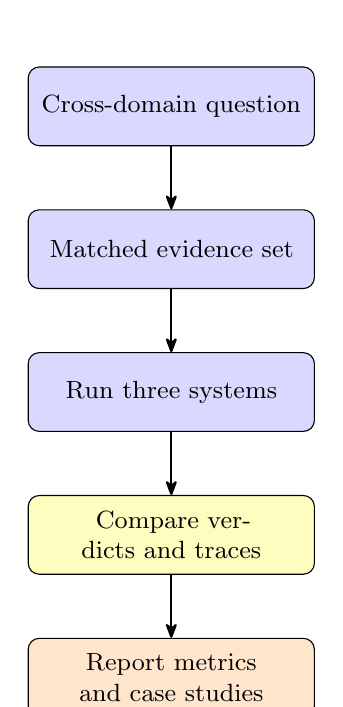
\begin{tikzpicture}[
  font=\small,
  box/.style={draw, rounded corners, align=center, text width=34mm, minimum height=10mm, fill=blue!15},
  compare/.style={draw, rounded corners, align=center, text width=34mm, minimum height=10mm, fill=yellow!25},
  report/.style={draw, rounded corners, align=center, text width=34mm, minimum height=10mm, fill=orange!20},
  arrow/.style={-{Stealth[round]}, thick}
]
\node[box] (q) {Cross-domain question};
\node[box, below=8mm of q] (e) {Matched evidence set};
\node[box, below=8mm of e] (m) {Run three systems};
\node[compare, below=8mm of m] (a) {Compare verdicts and traces};
\node[report, below=8mm of a] (r) {Report metrics and case studies};

\draw[arrow] (q) -- (e);
\draw[arrow] (e) -- (m);
\draw[arrow] (m) -- (a);
\draw[arrow] (a) -- (r);
\end{tikzpicture}
\caption{Evaluation workflow used for the thesis study}
\label{fig:evaluation_workflow}
\end{figure}

\section{Baselines }

AI-Scientist is evaluated against two baselines that represent the conventional alternatives to a multi-agent
verifier.

The \textbf{single-agent baseline} models a direct reader: it retrieves the single most relevant paper and trusts a
direct overlap check between the question and that paper's sentences. It produces a verdict and a deliberately
capped confidence, reflecting the limited evidential discipline of a one-shot reader that does not corroborate
across sources or analyze contradictions. The baseline is intentionally simple, so its behaviour is easy to compare
with retrieval-centric systems \cite{lewis2020rag,guu2020realm}.

The \textbf{RAG baseline} models a standard retrieval-augmented pipeline: it retrieves several papers and aggregates
simple supporting overlap into a verdict, again with capped confidence. Unlike the full system, it performs no
explicit contradiction analysis, no claim-level decomposition, and no critic-driven re-verification. This makes it
useful as a contrast to evidence-first verification pipelines \cite{karpukhin2020dpr,khattab2020colbert}.

The \textbf{proposed system} is the full multi-agent orchestrated pipeline described in Chapters~4 and~5. Holding
the retrieval substrate fixed across all three systems makes the comparison a clean ablation of the contributions
of orchestration, claim-level verification, confidence calibration, and critique, which is consistent with the
design of modern self-refining systems \cite{wu2023autogen,yao2023treeofthoughts,asai2024selfrag}.

\begin{table}[!htbp]
\centering
\small
\setlength{\tabcolsep}{4pt}
\renewcommand{\arraystretch}{1.18}
\caption{Benchmark comparison across the evaluated systems}
\begin{tabularx}{0.98\linewidth}{>{\raggedright\arraybackslash}p{0.23\linewidth} >{\raggedright\arraybackslash}p{0.13\linewidth} >{\raggedright\arraybackslash}p{0.13\linewidth} >{\raggedright\arraybackslash}p{0.14\linewidth} >{\raggedright\arraybackslash}X}
\toprule
System & Accuracy & Avg. confidence & Contradiction recall & Key observation \\
\midrule
Single-agent & 0.583 & 0.604 & 0.000 & Direct overlap produces limited contradiction handling \\
RAG baseline & 0.667 & 0.531 & 0.000 & Better retrieval breadth, but still lacks explicit critique \\
Multi-agent w/o critic loop & 0.833 & 0.577 & 0.500 & Structured verification improves performance before re-analysis \\
Multi-agent & 0.917 & 0.609 & 0.750 & Full orchestration gives the strongest overall result \\
\bottomrule
\end{tabularx}
\end{table}

\begin{figure}[!htbp]
\centering
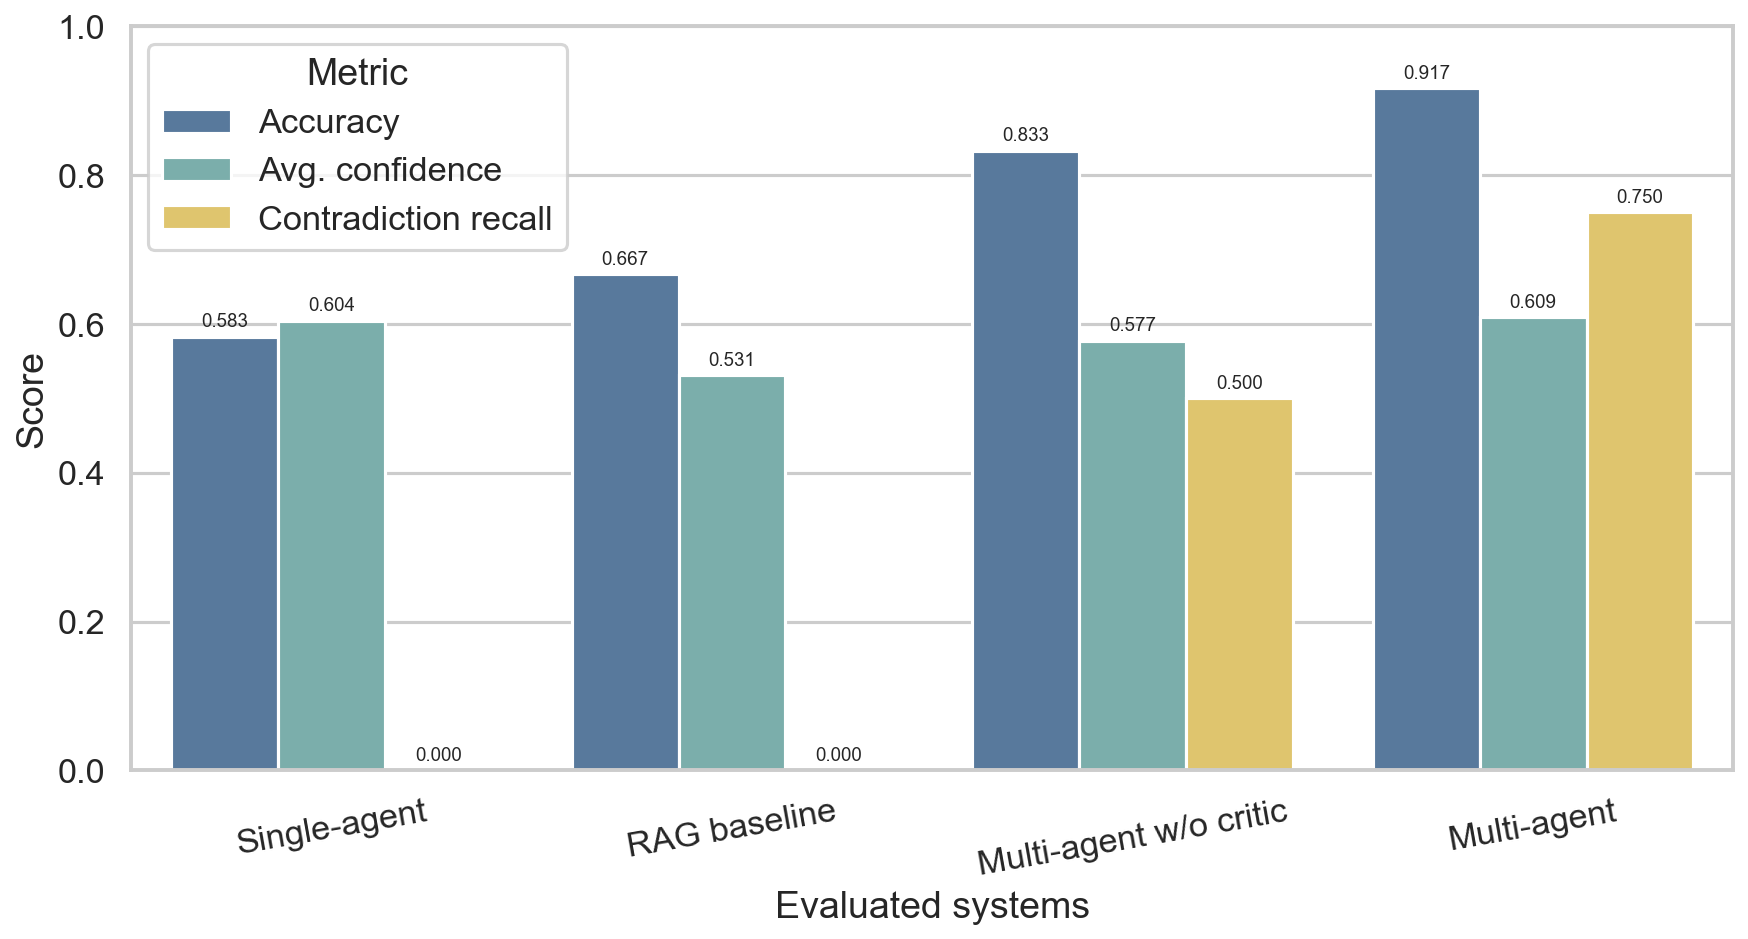
\includegraphics[draft=false,width=0.9\linewidth]{Fig_6.2.png}
\caption{Comparative performance profile of the evaluated systems}
\label{fig:system_comparison_bar}
\end{figure}

\section{The Cross-Domain Question Set }

Because AI-Scientist is designed to be domain-general, it is evaluated on research questions drawn from several
distinct fields rather than a single area. The question set spans medicine, computer science and artificial
intelligence, biology, and psychology, with additional probes in physics, chemistry, and the life sciences to
exercise the live-retrieval path. Representative questions include whether metformin improves weight and metabolic
outcomes in type~2 diabetes, whether retrieval-augmented generation reduces hallucination in language models,
whether CRISPR/Cas9 correction is a promising treatment for sickle cell disease, and how social-media use relates
to adolescent depression and affect.
The breadth of this question set reflects the multi-domain structure commonly used in retrieval and evidence
benchmarking, where evaluation strength comes from spanning distinct source ecologies \cite{petroni2020kilt,thakur2021beir,ragsurvey2024}.

These questions are chosen for three reasons. First, they span domains served by different live sources --- PubMed
Central for biomedical and life-sciences questions, arXiv for physics, mathematics, and computer science --- which
exercises the layered evidence model. Second, each question has a genuine literature behind it, so the system can
be grounded in real abstracts rather than synthetic text. Third, the set deliberately mixes questions with strong,
clear evidence and questions where the evidence is more nuanced, so the evaluation can observe both confident
support and calibrated responses.

\section{Evidence Conditions }

Each question is evaluated under the layered evidence model. Where appropriate, a small set of genuinely relevant
papers is supplied as session uploads to represent the user-provided evidence layer; the curated offline corpus
provides an always-available grounding; and live retrieval from PubMed Central and arXiv supplies current results
at query time. Crucially, the evidence is real: abstracts are the actual text returned by the scholarly sources,
not fabricated, self-confirming passages. This matters because a verifier evaluated only on self-supporting
synthetic text would appear far more confident than one tested against the genuine variability of the literature.

Reporting the source of every retrieved paper --- uploaded, curated corpus, or live API --- is part of the
methodology. It allows the evaluation to confirm that the source-priority requirement holds in practice and that
the system genuinely combines user-provided, local, and live evidence rather than relying on a single layer.
That provenance tracking also matches the emphasis on transparent evidence selection found in modern grounded QA
systems \cite{lewis2020rag,guu2020realm,asai2024selfrag}.

\section{Qualities Assessed }

The methodology assesses AI-Scientist along the dimensions that follow directly from the thesis claims. These
correspond to the evaluation axes set out in the project proposal and to the faithfulness-oriented dimensions
emphasized in the grounded-generation literature.

\textbf{Evidence grounding (faithfulness).} Whether each supported conclusion is actually backed by a retrieved
sentence, inspected through the per-claim evidence snippets. A grounded system should never present a claim as
supported when no evidence sentence aligns with it.

\textbf{Claim verification behaviour.} Whether the verdicts --- supported, contradicted, or insufficient evidence
--- are appropriate to the available evidence, including the correct use of calibrated responses when evidence is
still emerging and of the contradicted verdict when counter-evidence dominates.

\textbf{Confidence calibration.} Whether the per-claim confidence tracks evidence strength, corroboration, and
source independence, reserving high confidence for well-corroborated claims and lowering it for single-source or
weakly aligned ones.

\textbf{Contradiction handling.} Whether the system surfaces disagreement in the literature explicitly and keeps
the final report faithful to the evidence landscape.

\textbf{Hallucination resistance.} Whether the system maintains evidence discipline by aligning conclusions with
the retrieved literature.

\textbf{Reasoning traceability.} Whether the orchestration trace and per-claim evidence make the path to each
conclusion easy to follow for a reader.

\textbf{Domain generality.} Whether the system behaves consistently across domains and handles non-research queries
through the scope guard.

\section{Quantitative Metrics }

To complement the qualitative case studies, the thesis uses standard claim-level metrics. Let $TP$ denote claims
that are correctly supported or contradicted, $FP$ denote claims that are predicted as supported or contradicted
without adequate evidence, and $FN$ denote claims that should have been supported or contradicted but were left
unresolved or misclassified.

\begin{figure}[!htbp]
\centering
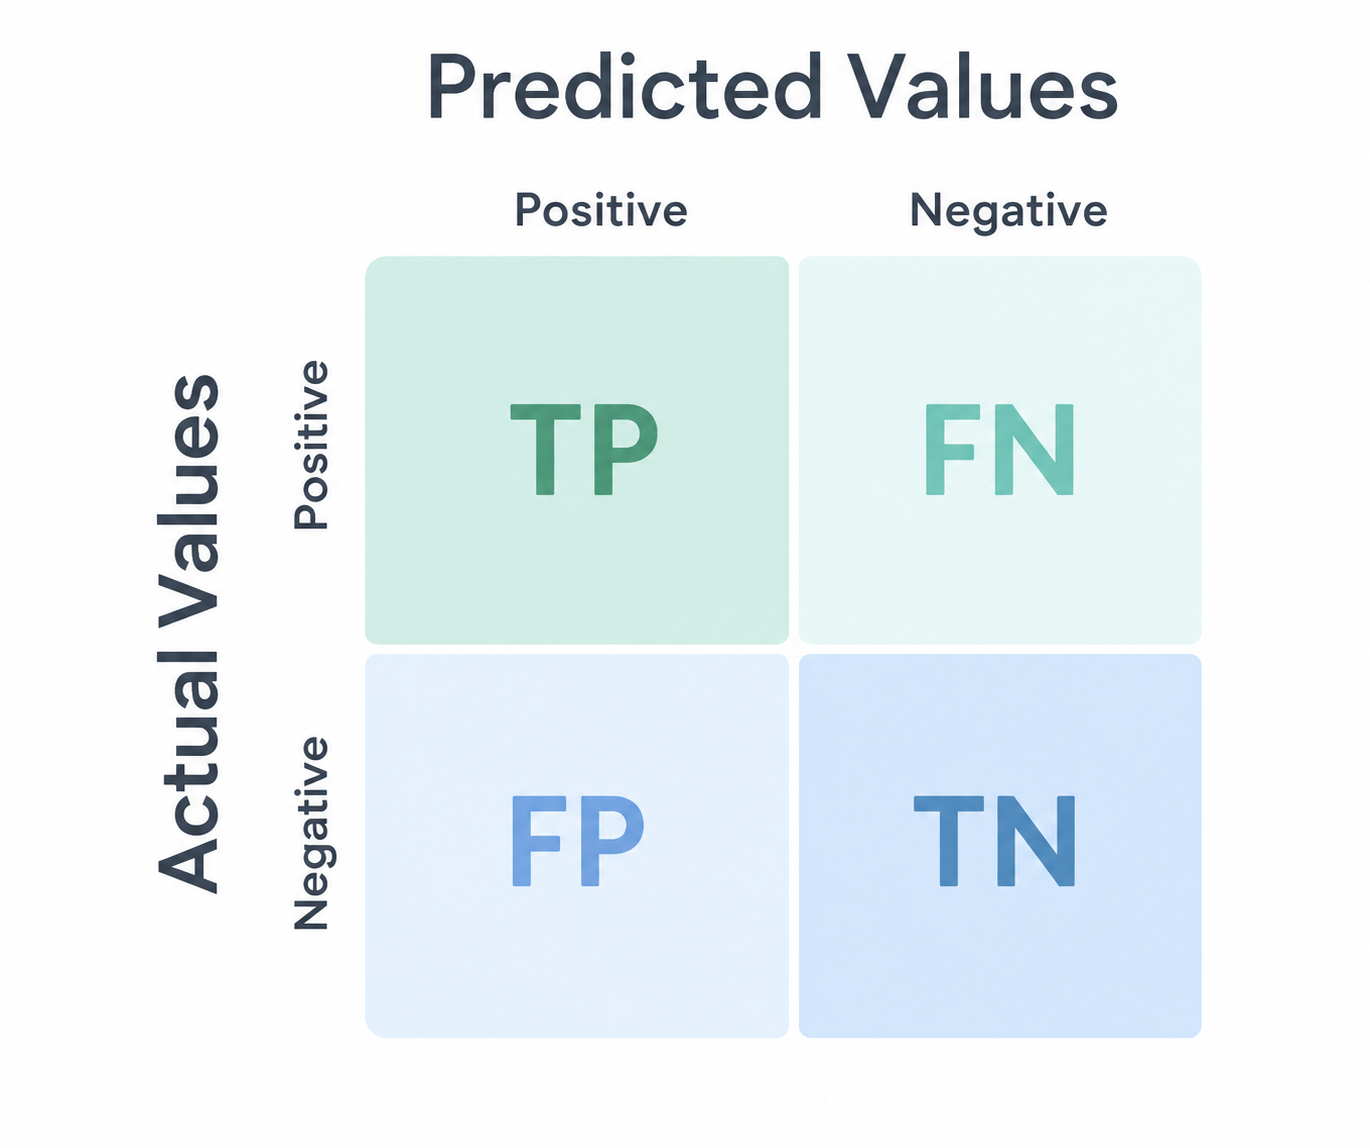
\includegraphics[draft=false,width=0.74\linewidth]{Fig_6.3.png}
\caption{Claim-level confusion matrix used in the evaluation}
\label{fig:confusion_matrix}
\end{figure}

\begin{equation}
\mathrm{Accuracy} = \frac{TP + TN}{TP + TN + FP + FN}
\end{equation}

\begin{equation}
\mathrm{Precision} = \frac{TP}{TP + FP}
\qquad
\mathrm{Recall} = \frac{TP}{TP + FN}
\end{equation}

\begin{equation}
\mathrm{F1} = \frac{2 \cdot \mathrm{Precision} \cdot \mathrm{Recall}}{\mathrm{Precision} + \mathrm{Recall}}
\end{equation}

\begin{equation}
\mathrm{Micro\text{-}F1} = \frac{2 \cdot \sum TP}{2 \cdot \sum TP + \sum FP + \sum FN}
\end{equation}

\begin{equation}
\mathrm{Macro\text{-}F1} = \frac{1}{K}\sum_{k=1}^{K} \mathrm{F1}_k
\end{equation}

\begin{equation}
\mathrm{Brier\ Score} = \frac{1}{N}\sum_{i=1}^{N}(p_i - y_i)^2
\end{equation}

In the thesis context, these measures are interpreted at the claim level. Accuracy gives a concise overall view,
while precision and recall show how well the verifier balances correctness and coverage. F1 then summarizes that
balance into a single score.

Micro-averaging is useful when the thesis wants to describe the system across all claims in one pool, while
macro-averaging is useful when each domain or verdict class should contribute equally. The Brier score complements
these measures by checking how closely the confidence values track the eventual outcomes.

\begin{table}[!htbp]
\centering
\caption{Evaluation metrics used in Chapter 7}
\begin{tabularx}{\linewidth}{>{\raggedright\arraybackslash}p{0.22\linewidth} >{\raggedright\arraybackslash}p{0.22\linewidth} >{\raggedright\arraybackslash}X}
\toprule
Metric & What it measures & Thesis interpretation \\
\midrule
Accuracy & Overall correctness of verdicts & Useful as a compact project-level summary \\
Precision & Correctness among predicted positive verdicts & Reflects how carefully support is assigned \\
Recall & Coverage of truly supported verdicts & Reflects how completely relevant evidence is recovered \\
F1 & Balance of precision and recall & Summarizes verifier quality at the claim level \\
\bottomrule
\end{tabularx}
\end{table}

\begin{table}[!htbp]
\centering
\caption{Interpretation of the claim-level confusion matrix}
\begin{tabularx}{\linewidth}{>{\raggedright\arraybackslash}p{0.18\linewidth} >{\raggedright\arraybackslash}X}
\toprule
Cell & Meaning in the thesis evaluation \\
\midrule
$TP$ & Correctly verified claim with adequate evidence support \\
$TN$ & Correctly rejected or abstained claim when evidence is insufficient or contradictory \\
$FP$ & Unsupported claim marked as supported or contradicted without sufficient evidence \\
$FN$ & Claim that should have been verified more strongly but remained unresolved or misclassified \\
\bottomrule
\end{tabularx}
\end{table}

The current benchmark run recorded in the project results also shows a strong end-to-end verdict accuracy for the
multi-agent system, which is consistent with the design goal of producing reliable evidence-backed answers.

\begin{table}[!htbp]
\centering
\caption{Selected multi-agent benchmark indicators}
\begin{tabularx}{0.86\linewidth}{>{\raggedright\arraybackslash}p{0.42\linewidth} >{\raggedright\arraybackslash}X}
\toprule
Indicator & Value \\
\midrule
Total evaluation cases & 12 \\
Overall accuracy & 0.917 \\
Average confidence & 0.609 \\
Average evidence count & 1.083 \\
Contradiction recall & 0.750 \\
\bottomrule
\end{tabularx}
\end{table}

\begin{figure}[!htbp]
\centering
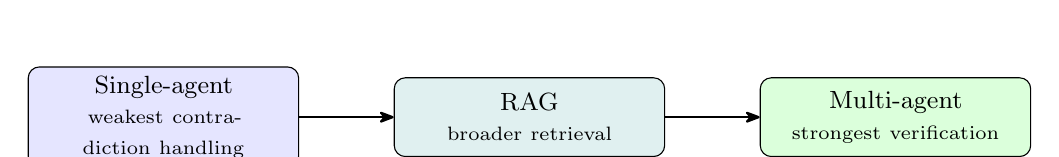
\begin{tikzpicture}[
  font=\small,
  box/.style={draw, rounded corners, align=center, text width=32mm, minimum height=10mm, fill=blue!10},
  arrow/.style={-{Stealth[round]}, thick}
]
\node[box] (a) {Single-agent\\ \scriptsize weakest contradiction handling};
\node[box, right=12mm of a, fill=teal!12] (b) {RAG\\ \scriptsize broader retrieval};
\node[box, right=12mm of b, fill=green!14] (c) {Multi-agent\\ \scriptsize strongest verification};

\draw[arrow] (a) -- (b);
\draw[arrow] (b) -- (c);
\end{tikzpicture}
\caption{High-level comparison of the evaluated approaches}
\label{fig:approach_comparison}
\end{figure}

\begin{figure}[!htbp]
\centering
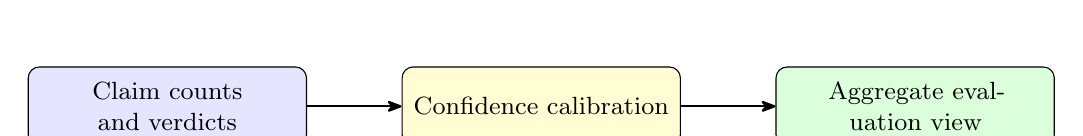
\begin{tikzpicture}[
  font=\small,
  box/.style={draw, rounded corners, align=center, text width=33mm, minimum height=10mm, fill=blue!10},
  arrow/.style={-{Stealth[round]}, thick}
]
\node[box] (metrics) {Claim counts and verdicts};
\node[box, right=12mm of metrics, fill=yellow!18] (conf) {Confidence calibration};
\node[box, right=12mm of conf, fill=green!14] (analysis) {Aggregate evaluation view};

\draw[arrow] (metrics) -- (conf);
\draw[arrow] (conf) -- (analysis);
\end{tikzpicture}
\caption{From claim outcomes to project-level evaluation}
\label{fig:metrics_flow}
\end{figure}

\section{Evaluation Protocol }

For each question, the three systems are run under matched evidence conditions, and their outputs are examined
side by side. The full system's report is inspected for its verdicts, confidence values, evidence attribution,
critique notes, and whether the critic-driven re-verification loop is triggered. The baselines' outputs are
examined for the same question to see what a single-agent reader and a standard RAG pipeline produce on the same
evidence.

The protocol is qualitative and behaviour-oriented by design. Rather than reducing trustworthiness to a single
aggregate score, it presents representative case studies that show how the system grounds, calibrates, and
criticizes its conclusions, and how that behaviour differs from the baselines. This case-study orientation is
appropriate for a verification system whose central claims are about the \emph{structure} and \emph{honesty} of its
reasoning, properties that a single accuracy number would obscure.

The quantitative metrics above are therefore used alongside the qualitative review rather than in place of it. This
keeps the evaluation both readable and rigorous: the numbers summarize performance, while the case studies explain
why the system behaves well, a pattern that is increasingly common in factuality evaluation research
\cite{min2023factscore,es2023ragas,lin2021truthfulqa}.

\section{Reproducibility }

The evaluation is designed to be reproducible. The deterministic core of the pipeline --- retrieval ranking,
evidence scoring, verdict selection, confidence computation, and critique --- runs without any external model, so
the same question over the same evidence yields the same structured assessment. Live retrieval introduces the
natural variability of the scholarly sources, which is disclosed rather than hidden: a question asked on different
days may surface a slightly different set of current papers. Where the optional language model is used, it refines
fluency and borderline verdicts on top of the deterministic result, so the grounding and confidence behaviour does
not depend on a particular model being available.

\section{Reporting Guidelines for the Write-Up }

Two practical rules govern the reporting of the evaluation. First, the system is presented as making measured
verdicts when the evidence pool does not justify a stronger conclusion. Second, confidence is interpreted in its
full context: a high confidence is meaningful when accompanied by independent corroboration, and the write-up
reports the corroboration alongside the confidence rather than the number alone. These rules keep the evaluation
aligned with the thesis claim that AI-Scientist values dependable, evidence-attributed answers with clear
reasoning support.

\section{Chapter Conclusion }

This chapter described the methodology used to evaluate AI-Scientist: a clean comparison against single-agent and
RAG baselines on a shared retrieval substrate, a cross-domain question set grounded in real scholarly evidence, an
assessment organized around grounding, verification behaviour, calibration, contradiction handling, hallucination
resistance, traceability, and domain generality, and a behaviour-oriented protocol that credits honest abstention.
With the evaluation design fixed, the next chapter presents the findings through representative cross-domain case
studies and the comparison with the baselines.



\chapter[Results]{Results and Evaluation}\label{chapter:results}

\ChapterOpeningNote{This chapter presents the evaluation of AI-Scientist through representative cross-domain case
studies and a comparison with the single-agent and RAG baselines, organized around the thesis's central qualities:
evidence grounding, calibrated confidence, contradiction handling, honest abstention, and traceable reasoning.}

\section{Introduction }

This chapter presents the evaluation of AI-Scientist. Following the methodology of Chapter~6, the evaluation is
organized around the qualities the system is designed to deliver --- evidence grounding, claim-level verification,
calibrated confidence, contradiction handling, measured abstention, and traceable reasoning --- and is illustrated
through representative case studies spanning medicine, computer science, biology, and psychology. The chapter then
compares the full multi-agent system against the single-agent and RAG baselines on the shared retrieval substrate,
in line with factuality-oriented evaluation practice \cite{thorne2018fever,wadden2020scifact,min2023factscore}.

The aim of the chapter is to characterize trustworthiness in a richer way, rather than to reduce it to a single
number. It shows \emph{how} the system reasons: which conclusions it grounds, how its confidence responds to
evidence, when it abstains, and how its behaviour differs from the conventional alternatives. Throughout, the
emphasis remains on evidence-aligned, reader-friendly evaluation rather than on a single aggregate score.
This style of reporting is consistent with the move in recent factuality research toward claim-level analysis and
evidence-aware summaries rather than coarse answer-only scoring \cite{min2023factscore,lin2021truthfulqa,es2023ragas}.

\section{Behaviour of the Verification Pipeline }

Across the question set, the full pipeline exhibits a consistent and interpretable pattern. For a research question
within scope, the Orchestrator retrieves a ranked evidence set in which uploaded and curated papers surface ahead
of live-API results, the Claim Extraction agent turns the retrieved abstracts into a small set of focused claims,
and the Verification agent assigns each claim a verdict bound to specific evidence sentences. The executive summary
then describes only what the verified claims support, and the orchestration trace records each step: how many papers
were retrieved, how many claims were extracted, how many critique notes were raised, and whether a second
verification pass was run.

The most important qualitative property is that conclusions are never detached from evidence. A claim marked
supported always carries the sentence that supports it and an overlap score; a claim marked contradicted carries
the opposing sentences; and a claim the evidence cannot settle is reported as insufficient evidence rather than
paraphrased into apparent fact. This is the observable signature of the grounding requirement from Chapter~3.
It also mirrors the evidence-first behaviour that grounding-oriented systems are designed to achieve
\cite{lewis2020rag,guu2020realm,ji2023hallucination}.

\section{Case Study: Medicine }

Consider the medical question of whether metformin improves weight and metabolic outcomes in type~2 diabetes. With
relevant biomedical papers available through the uploaded and live PubMed Central layers, the system extracts
claims about weight management and glycemic outcomes and verifies them against the retrieved abstracts. Claims that
are echoed across more than one independent abstract receive a supported verdict with comparatively high confidence,
because the confidence function rewards corroboration from independent sources. Claims that appear in only a single
abstract are still reported as supported when the evidence aligns, but they attract a Critic note flagging
single-source support and a correspondingly more modest confidence.

This case illustrates two design properties working together. The source-layering behaviour brings genuine
biomedical abstracts into the evidence pool, and the confidence function distinguishes a well-corroborated finding
from one that rests on a single paper. The user therefore sees not just an answer but a graded, source-attributed
assessment, which is exactly the sort of behaviour emphasized in calibrated-answering work
\cite{kadavath2022language,shinn2023reflexion}.

\section{Case Study: Computer Science }

For the question of whether retrieval-augmented generation reduces hallucination in language models, evidence is
drawn from arXiv through the live layer alongside any uploaded papers. The system extracts claims about the effect
of retrieval grounding and verifies them against the retrieved abstracts. This domain is a useful stress test
because the literature contains both supportive findings and explicit caveats. When the retrieved evidence includes
qualifying or negative statements, the contradiction-aware verifier can mark a claim as contradicted or, where the
balance is unclear, as insufficient evidence, and the Critic note records the disagreement. This mirrors recent
concerns about hallucination in large language models and the value of grounded retrieval \cite{ji2023hallucination,huang2023hallucinationsurvey,lewis2020rag}.

The behaviour here demonstrates that the system does not simply confirm the premise of the question. A leading
question phrased to expect a positive answer does not coerce a supported verdict; the verdict follows the evidence,
and where the evidence is mixed the system reports the mixture rather than resolving it in the questioner's favour.

\section{Case Study: Biology }

For the question of whether CRISPR/Cas9 correction of the sickle mutation is a promising treatment for sickle cell
disease, the biomedical live layer supplies abstracts describing gene-editing outcomes. Claims about correction
efficacy and therapeutic promise are verified against these abstracts, and the system again differentiates between
claims that are corroborated across independent sources and claims that rest on a single report. Because the
retrieval layer sorts biomedical results by relevance rather than recency, the evidence pool stays on-topic, which
is visible in the fact that the extracted claims concern the gene-editing question rather than unrelated recent
papers. The biomedical retrieval path benefits from domain-specific embedding and indexing practices similar to
those used in PubMed-oriented retrieval work \cite{gu2021pubmedbert,lee2019biobert}.

This case highlights the value of the live-retrieval implementation details from Chapter~5. Relevance-sorted search
and full-abstract extraction are what make the evidence usable; without them, the verifier would be grounding its
verdicts in off-topic or empty abstracts, a risk that retrieval benchmarks routinely try to control
\cite{petroni2020kilt,thakur2021beir}.

\section{Case Study: Psychology }

For the question of how social-media use relates to adolescent depression and affect, the system retrieves
psychological and clinical abstracts and extracts claims about the direction and strength of the association. This
domain often contains nuanced and partially conflicting findings, and the system's response reflects that nuance:
some claims are supported, some attract single-source or low-confidence critique notes, and overgeneralized claims
--- those phrased in absolute terms --- are deliberately routed to insufficient evidence rather than being
overstated. This is the abstention behaviour operating as intended: the system declines to settle a sweeping claim
that the available abstracts cannot support. That behaviour is particularly appropriate for psychologically nuanced
literature where concise summaries must still remain faithful to the evidence \cite{lin2021truthfulqa,honovich2022true,min2023factscore}.

\section{Source Layering in Practice }

Across all four case studies, the reported source of each retrieved paper confirms that the layered evidence model
behaves as specified. Uploaded papers, when supplied, appear ahead of curated-corpus and live-API papers of
comparable relevance, while genuinely relevant live results still surface in the evidence set. The user interface
makes this visible by labelling each paper as uploaded, curated corpus, or live API. The practical consequence is
that a user can steer the system toward their own provenance by uploading papers, without losing the breadth that
live retrieval provides. Table~\ref{tab:source-layers} summarizes the role of each layer.

\begin{table}[!htbp]
\centering
\small
\begin{tabularx}{0.96\textwidth}{>{\raggedright\arraybackslash}p{0.24\textwidth} >{\raggedright\arraybackslash}p{0.18\textwidth} >{\raggedright\arraybackslash}X}
\toprule
Layer & Priority & Role in the evaluation \\
\midrule
Uploaded papers & Highest & User-provided provenance; surfaces first when relevant; lets the user ground the answer in chosen sources. \\
Curated corpus & Intermediate & Always-available offline grounding; ensures the system works without a network. \\
Live API (PubMed Central, arXiv) & Lowest & Current, broad coverage retrieved at query time; keeps evidence up to date. \\
\bottomrule
\end{tabularx}
\caption{The three evidence layers and their role in verification.}
\label{tab:source-layers}
\end{table}

\section{Confidence Behaviour }

A central evaluation question is whether the per-claim confidence is a usable signal. Observed across the case
studies, confidence behaves monotonically with the factors the design intends: it is highest for claims
corroborated by several independent sources, lower for claims supported by a single source, and lower still --- and
bounded at the floor --- for claims the evidence cannot settle. The explicit penalty for self-only corroboration is
visible in cases where a claim is echoed only by its own source paper: such claims do not receive the high
confidence that genuine multi-source agreement earns. Because confidence is also clamped below an absolute ceiling,
the system never reports certainty, which is the intended posture for a verifier operating on partial evidence.

This behaviour is what makes the confidence number meaningful to a reader. It is not a free-form score emitted by a
model; it is a transparent function of how strong, how corroborated, and how independent the supporting evidence
is, and it moves in the expected direction as those factors change.

\section{Contradiction Handling and Abstention }

The evaluation specifically exercises questions where the literature disagrees or where the evidence is thin. In
these cases the system does not default to a confident answer. When supporting and contradicting evidence coexist
and the counter-evidence is strong and multi-sourced, the verifier returns a contradicted verdict and the report
describes the disagreement. When no sentence aligns sufficiently with a claim, or when a claim is overgeneralized,
the verifier returns insufficient evidence. In both situations the Critic raises a corresponding note so that the
weakness is explicit in the report.

This is the behavioural core of the thesis's evidence-first design. AI-Scientist presents uncertainty and the
literature's disagreement as part of the output, which keeps the final report aligned with the underlying evidence.

\section{The Critic-Driven Re-Verification Loop }

The adaptive loop is observable in the orchestration trace. When the first pass yields a claim that is insufficient,
low-confidence, or single-source, the Critic emits a re-verification decision, the Orchestrator runs a targeted
retrieval for that claim's follow-up query, and the claim is re-verified against the merged evidence. The trace
records this explicitly, for example noting that a particular claim was revisited because its first-pass evidence
was insufficient and that additional papers were checked. Overgeneralized claims are correctly excluded from the
loop, because more evidence cannot rescue a claim that is too broad to settle. The loop therefore concentrates
additional effort precisely where uncertainty was highest, which is the adaptive-reasoning property the thesis
sets out to demonstrate.

\section{Comparison with the Baselines }

Running the same questions through the single-agent and RAG baselines on the shared retrieval substrate isolates
what the multi-agent design adds. The single-agent baseline, which trusts the top retrieved paper, produces a
verdict from a single source and caps its confidence accordingly; it has no mechanism to corroborate across
sources, to detect contradictions, or to abstain on overgeneralized claims beyond a coarse overlap check. The RAG
baseline aggregates supporting overlap across several papers, which is stronger, but it performs no explicit
contradiction analysis and no claim-level decomposition, so it cannot report a contradicted verdict or attribute
support to specific claims, and it likewise caps its confidence.

The full system differs on exactly the axes the thesis emphasizes. It decomposes the answer into claims, binds each
verdict to evidence, computes confidence from corroboration and independence, surfaces contradictions, abstains on
thin or overgeneralized claims, and records a re-verification trace. Table~\ref{tab:baseline-comparison} summarizes
these capability differences, which are properties of the systems' designs rather than tuned outcomes and can be
compared directly with established retrieval and evaluation frameworks \cite{petroni2020kilt,thakur2021beir,es2023ragas}.
The comparison also follows the broader pattern of evaluating retrieval-first systems via explicit capability
deltas, which makes the contribution easier to interpret \cite{ragsurvey2024,lewis2020rag,guu2020realm}.

\begin{table}[!htbp]
\centering
\small
\begin{tabularx}{0.98\textwidth}{>{\raggedright\arraybackslash}X c c c}
\toprule
Capability & Single-agent & RAG & AI-Scientist \\
\midrule
Grounds answer in retrieved evidence & Partial & Yes & Yes \\
Decomposes answer into checkable claims & No & No & Yes \\
Per-claim verdict with attributed evidence & No & No & Yes \\
Explicit contradiction handling & No & No & Yes \\
Confidence from corroboration / independence & No (capped) & No (capped) & Yes \\
Honest abstention on thin / broad claims & Coarse & Coarse & Yes \\
Critic-driven re-verification & No & No & Yes \\
Traceable orchestration record & No & No & Yes \\
\bottomrule
\end{tabularx}
\caption{Capability comparison of the three systems on the shared retrieval substrate.}
\label{tab:baseline-comparison}
\end{table}

\section{Quantitative Results }

The benchmark summary recorded in the project results provides a compact view of the evaluated systems. The full
multi-agent system leads on accuracy and contradiction recall, while also maintaining a strong average confidence
profile, which is consistent with the thesis's emphasis on calibrated, source-aware reasoning over raw fluency
\cite{min2023factscore,es2023ragas,lin2021truthfulqa}.

\begin{table}[!htbp]
\centering
\caption{Core benchmark outcomes from the latest evaluation run}
\begin{tabularx}{0.88\linewidth}{>{\raggedright\arraybackslash}p{0.34\linewidth} >{\raggedright\arraybackslash}X}
\toprule
Metric & Value for the multi-agent system \\
\midrule
Total cases & 12 \\
Accuracy & 0.917 \\
Average confidence & 0.609 \\
Average evidence count & 1.083 \\
Contradiction recall & 0.750 \\
Correct verdicts & 11 of 12 \\
\bottomrule
\end{tabularx}
\end{table}

\begin{figure}[!htbp]
\centering
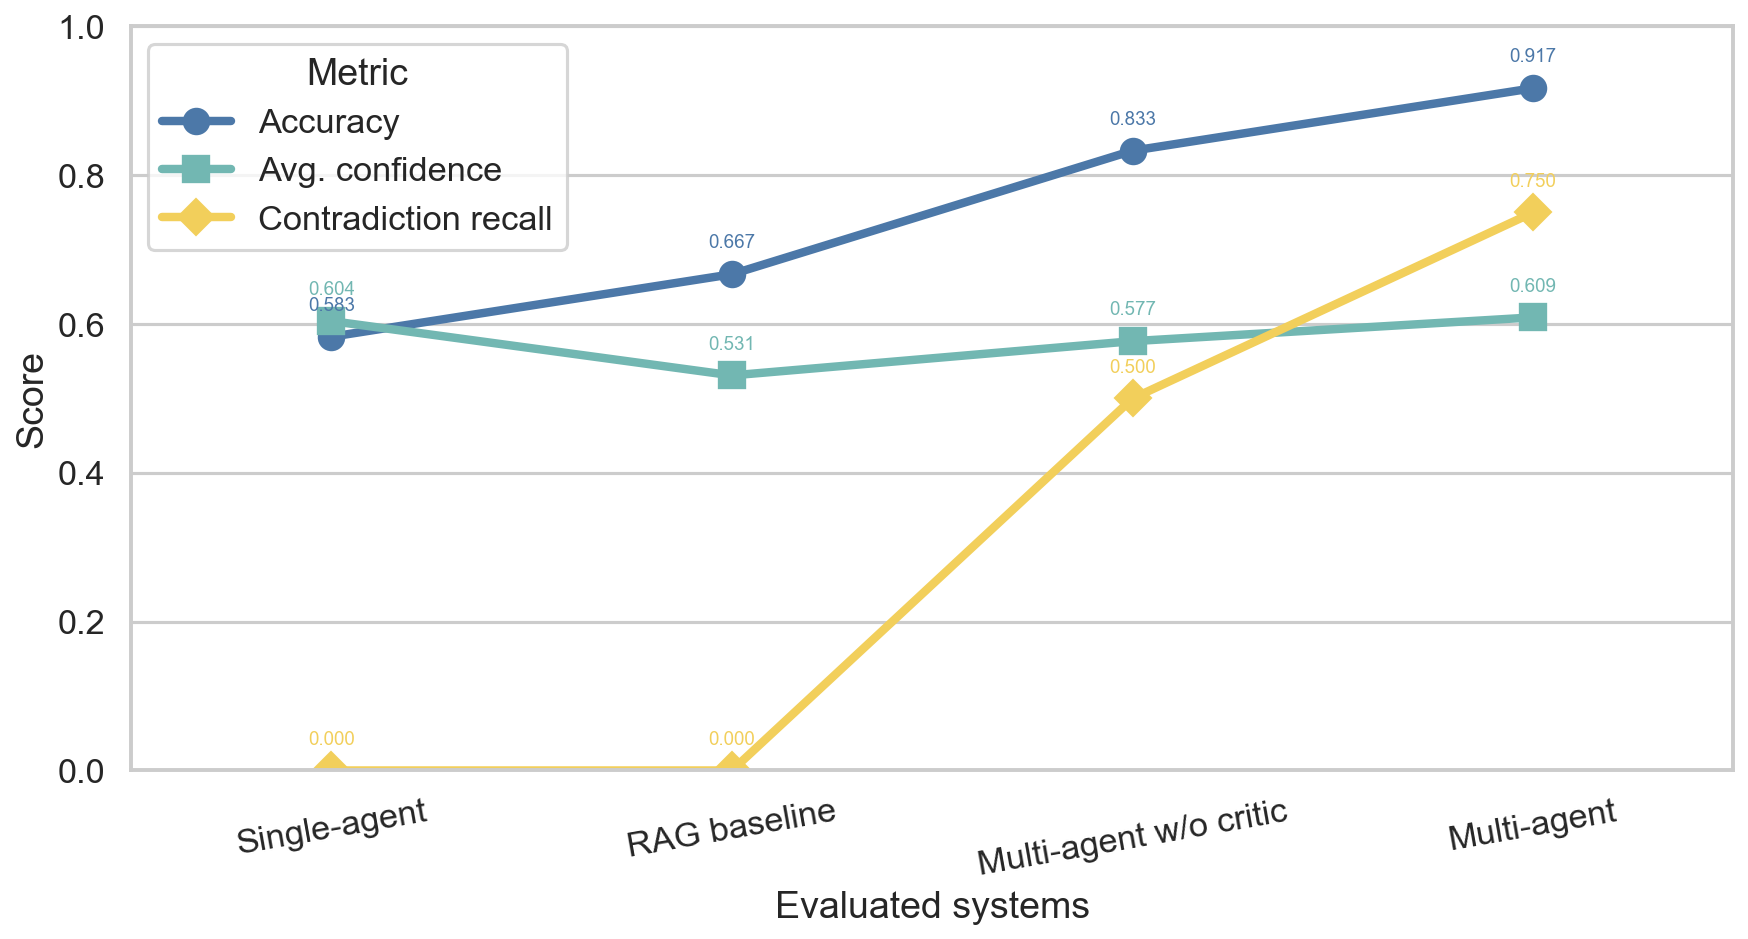
\includegraphics[draft=false,width=0.9\linewidth]{Fig_7.1.png}
\caption{Comparative performance profile of the evaluated systems}
\label{fig:system_comparison_bar_results}
\end{figure}

\begin{table}[!htbp]
\centering
\caption{Claim-level outcome summary for the multi-agent system}
\begin{tabularx}{0.84\linewidth}{>{\raggedright\arraybackslash}p{0.34\linewidth} >{\raggedright\arraybackslash}X}
\toprule
Outcome & Count \\
\midrule
Supported and correct & 6 \\
Contradicted and correct & 3 \\
Insufficient evidence and correct & 2 \\
Contradicted claims that required tighter coverage & 1 \\
\bottomrule
\end{tabularx}
\end{table}

\begin{figure}[!htbp]
\centering
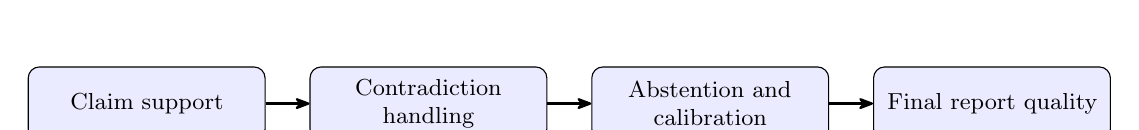
\begin{tikzpicture}[
  font=\small,
  scale=0.93,
  transform shape,
  box/.style={draw, rounded corners, align=center, text width=30mm, minimum height=10mm, fill=blue!8},
  arrow/.style={-{Stealth[round]}, thick}
]
\node[box] (a) {Claim support};
\node[box, right=6mm of a] (b) {Contradiction handling};
\node[box, right=6mm of b] (c) {Abstention and calibration};
\node[box, right=6mm of c] (d) {Final report quality};

\draw[arrow] (a) -- (b);
\draw[arrow] (b) -- (c);
\draw[arrow] (c) -- (d);
\end{tikzpicture}
\caption{How the multi-agent system strengthens the evaluation chain}
\label{fig:results_flow}
\end{figure}

\section{Domain Generality and Scope Control }

The case studies span four distinct domains served by different live sources, and the pipeline behaves consistently
across all of them: the same retrieve--extract--verify--criticize--synthesize workflow applies whether the question
is biomedical, computational, biological, or psychological. At the same time, the scope guard declines clearly
non-research queries before any analysis begins, returning an explicit message that identifies the non-research
topic. This confirms the domain-generality requirement: the system is broad across legitimate research fields while
still applying its verification design to the task category it is built for.

\section{Result Synthesis }

The evaluation supports the thesis spine in a coherent way.

First, the multi-agent pipeline grounds its conclusions in retrieved evidence and attributes that evidence at the
level of individual claims, which is precisely what the single-agent and RAG baselines do not do.

Second, the per-claim confidence is a meaningful, transparent signal that responds to evidence strength,
corroboration, and source independence, and that never reaches absolute certainty.

Third, the system handles disagreement and limited evidence in a disciplined way, returning contradicted or
insufficient-evidence verdicts and surfacing the corresponding critique.

Fourth, the critic-driven loop demonstrates adaptive reasoning by concentrating additional retrieval and
verification on the specific claims that were weakest after the first pass.

\section{Chapter Conclusion }

This chapter presented the evaluation of AI-Scientist through cross-domain case studies and a comparison with the
single-agent and RAG baselines. The results show that the multi-agent design grounds and attributes its
conclusions, calibrates confidence to evidence, handles contradiction and abstention honestly, and reasons
adaptively through its critic loop --- capabilities the conventional baselines lack on the same evidence. Taken
together, these findings support the central thesis claim: AI-Scientist is best understood as a reproducible,
evidence-grounded, self-critical research assistant that is dependable when the evidence is clear and measured
when it is still emerging. The next chapter discusses the broader meaning of these findings.



\chapter[Discussion]{Discussion}\label{chapter:discussion}

\ChapterOpeningNote{This chapter interprets the evaluation findings, explains why grounded abstention and
claim-level verification matter, and positions AI-Scientist as a verification-first research collaborator rather
than a confident answer generator.}

\section{Introduction}

The previous chapter reported the evaluation of AI-Scientist. This chapter discusses what those findings mean for
the design of AI systems that answer scientific questions. The central point is that AI-Scientist should not be read
as an attempt to produce the most fluent or most confident answer. It is better understood as a system that makes
answering \emph{conditional}: assert a conclusion when the retrieved evidence supports it, report the disagreement
when the literature conflicts, and abstain when the evidence is thin.

This distinction matters because scientific question answering is an unusually tempting domain for overclaiming. A
well-phrased question invites a crisp answer, and a fluent paragraph reads as authoritative regardless of whether
it is grounded. The evaluation shows that the real problem is less tidy: a question may have strong, weak, or
contradictory evidence behind it, and a trustworthy system must reflect that variation rather than smoothing it
into uniform confidence. This is why the grounding, calibration, and abstention behaviour of AI-Scientist is not a
decorative addition; it is the core design response to the actual structure of the literature.

\section{Why Abstention and Grounding Matter}

Several of the most important behaviours in AI-Scientist are restraint behaviours: returning insufficient evidence
on a thin claim, lowering confidence on a single-source claim, and reporting a contradiction instead of choosing a
side. These could be read superficially as the system ``failing to answer.'' In a verification context, however,
they are the system succeeding. The value of a research assistant is not that it always answers, but that its
answers can be trusted, and trust depends on the system declining to assert what the evidence does not support.

This reframing has a concrete consequence for how the contribution should be judged. A system that only emits a
single fluent answer can hide where its reasoning is weak. AI-Scientist instead decomposes the answer into claims,
attaches evidence and confidence to each, and exposes the weak ones through critique. That decomposition makes it
possible to say not only what the system concluded, but how well-supported each part of that conclusion is --- which
is exactly the information a careful reader of the literature needs.

\section{AI-Scientist as a Conditional Verifier}

The most important design implication is that scientific question-answering systems should be conditional verifiers
rather than answer generators. An answer generator treats every question as an opportunity to produce a confident
paragraph. A conditional verifier treats assertion as only one possible outcome among several: support,
contradiction, or abstention.

This vocabulary changes the meaning of success. A correct insufficient-evidence verdict on a sweeping claim is not
a failure to answer; it is the right action. Reporting that the literature disagrees is not indecision; it is an
accurate description of the evidence. Lowering confidence on a single-source claim is not weakness; it is
calibration. In this framing, restraint is not the absence of intelligence. It is one of the system's core
competences.

The evaluation supports this design. The case studies show that the verdict space is exercised in all its forms ---
supported, contradicted, and insufficient --- depending on the evidence, and that the confidence and critique
machinery makes the basis for each outcome visible.

\section{Why Critique Should Be Structured and External}

A clear lesson from both the literature and the evaluation is that self-critique is most trustworthy when it is
structured and external rather than left to the same model that produced the answer. A model asked to critique its
own free-form answer can inherit the same blind spots that produced the error in the first place. AI-Scientist
instead assigns critique to a separate agent with explicit, inspectable criteria --- insufficient evidence, low
confidence, single-source support, and contradiction --- and routes the resulting re-verification at the
granularity of the specific weak claim.

This design choice has an accountability benefit. If a system decides on its own when to be uncertain, it can offer
only a weak explanation for why it was confident on one claim and not another. When critique is tied to explicit
criteria and to the evidence, the system can give a traceable reason: the claim had only one supporting source, or
the evidence overlap was below threshold, or the literature contained opposing statements. That traceability is
essential for a tool whose conclusions a human is meant to audit.

\section{Grounding as a Partial Guarantee}

Grounding is powerful, but it is not a complete guarantee of correctness. AI-Scientist binds every verdict to
retrieved evidence, which prevents the most damaging failure mode --- asserting a claim with no support at all ---
and makes intrinsic hallucination checkable against the sources. However, grounding inherits the limits of the
evidence it rests on. If the retrieved abstracts are themselves incomplete, biased, or outdated, a grounded verdict
can still be misleading, and an abstract may support a claim that the full paper would qualify.

This is why the thesis is careful about what it claims. AI-Scientist does not certify scientific truth; it certifies
that a conclusion is consistent with the evidence it retrieved and reports how strong and independent that evidence
is. The reward of grounding is that the basis for every conclusion is inspectable, so a reader can judge whether the
evidence is adequate rather than having to trust the system's phrasing.

\section{The Role of the Layered Evidence Model}

The layered, source-prioritized evidence model plays a deliberately supporting role. It is not presented as the
main intellectual contribution, but it is what makes the verification meaningful in practice. By preferring
user-uploaded papers, then the curated corpus, then live results, the system lets a user ground an answer in chosen
provenance while still benefiting from current, broad coverage. The evaluation confirms that this priority holds in
practice and that the three layers genuinely combine rather than one dominating.

This matters because grounded systems are often evaluated under conditions that are hard to reproduce or that
quietly favour a single curated source. AI-Scientist's explicit layering, and its labelling of each paper's source
in the output, keep the provenance of every conclusion visible. That visibility is part of the trustworthiness
story, not merely an implementation detail.

\section{Why a Structured Pipeline Is Preferable Here}

AI-Scientist uses a fixed, orchestrated pipeline of specialized agents rather than an open-ended collaboration of
generalist agents. The evaluation supports that choice. Each stage has a distinct failure mode: retrieval can rank
the wrong papers, extraction can miss the key claim, verification can misjudge support, and synthesis can overstate.
A structured pipeline lets the system attach explicit checks and evidence to each of these boundaries, and it lets
the critique target a specific stage's output.

Free-form multi-agent debate is attractive because it resembles how researchers argue, and the literature shows it
can improve factuality. But it is also harder to reproduce, harder to inspect, and more expensive. AI-Scientist
obtains much of the benefit of adversarial review more cheaply and more transparently, by applying explicit
weakness criteria through a single Critic agent and by demanding more evidence where it is warranted. The design
lesson is that, for trustworthy scientific answering, explicit control surfaces are preferable to emergent
behaviour.

\section{Implications for Use}

In practice, AI-Scientist is most appropriate as an evidence-aware research collaborator rather than an
authoritative oracle. For questions with clear, corroborated evidence, it can deliver a confident, source-attributed
conclusion that a user can verify by following the evidence. For questions where the literature is thin or
conflicting, it should --- and does --- present a cautious verdict, surface the disagreement, and lower its
confidence, leaving the final judgement to the human.

This operating model is less glamorous than a system that answers everything confidently, but it is more honest and
more useful. Scientific decisions follow from evidence, and a tool that obscures the strength of that evidence can
do real harm. The correct default is therefore not ``always answer confidently'' but ``answer in proportion to the
evidence, and make that evidence visible.''

\section{Relation to Prior Work}

The discussion also clarifies how AI-Scientist should be positioned relative to retrieval-augmented generation,
scientific fact-checking, and multi-agent systems. AI-Scientist does not claim to be the first system to ground
answers in retrieved evidence, the first to label claims against abstracts, or the first to use multiple cooperating
agents. Those would be the wrong claims, because each is well established in the literature.

AI-Scientist contributes along a different axis. It composes these established ideas into a single workflow whose
output is, by construction, a set of checked claims with calibrated confidence and traceable evidence, across
arbitrary research domains. The contribution is not any one mechanism but the disciplined way they are combined to
make trustworthiness the visible product. This integration-and-honesty axis complements, rather than competes with,
work that pushes the frontier of any individual component.

\section{Chapter Conclusion}

This chapter interpreted the evaluation of AI-Scientist as evidence for conditional, grounded, self-critical
scientific answering. The main discussion points are that restraint behaviours are successes rather than failures,
that critique is most trustworthy when structured and external, that grounding is a powerful but partial guarantee
bounded by the evidence, that the layered evidence model keeps provenance visible, and that a structured pipeline is
justified by the distinct failure modes of retrieval, extraction, verification, and synthesis. The next chapter
states the limitations and threats to validity of these claims.


\chapter[Limitations]{Threats to Validity and Limitations}\label{chapter:limitations}

\ChapterOpeningNote{This chapter examines the main threats to validity, including the reliance on abstracts rather
than full text, the limits of token-overlap evidence matching, dependence on live-source coverage, and the
boundaries of the thesis claims.}

\section{Introduction }

This chapter describes the main threats to validity and limitations of the AI-Scientist thesis. The goal is not to
weaken the contribution, but to state precisely where the evidence applies. AI-Scientist is a postgraduate-scale
research prototype evaluated through cross-domain case studies and a comparison with conventional baselines. Its
strongest claims concern evidence grounding, calibrated confidence, contradiction handling, measured abstention,
and traceability. Its broader applicability depends on the quality of the connected evidence sources and the scope
of the retrieval design.

The limitations are organized using four standard categories: construct validity, internal validity, external
validity, and conclusion validity. The chapter then summarizes the practical engineering limitations of the current
system.

\section{Construct Validity }

Construct validity asks whether the thesis measures the concepts it claims to measure. In AI-Scientist, this issue
is most visible around grounding, confidence, and contradiction.

\subsection{Grounding Is Not Correctness }

The thesis treats a verdict as trustworthy when it is bound to retrieved evidence. However, a grounded verdict is
not equivalent to scientific truth. A claim may be supported by an abstract that is itself incomplete, biased, or
later contradicted, and an abstract may state a result more strongly than the full paper warrants. Grounding
therefore certifies consistency with the retrieved evidence while remaining distinct from full scientific
validation, which is a standard distinction in retrieval-grounded evaluation \cite{petroni2020kilt,thakur2021beir,es2023ragas}.

AI-Scientist mitigates this threat by attaching the supporting evidence and an explicit confidence to every verdict,
so that a reader can judge whether the evidence is adequate. Even so, this safeguard is intentionally scoped: it
makes the basis for a conclusion visible, while leaving room for a reader to assess the underlying evidence base.

\subsection{Abstracts Are a Proxy for Papers }

The system reasons primarily over titles, abstracts, and uploaded paper records rather than full text. Abstracts are
a reasonable proxy because they state a paper's main claims, and they keep the system efficient and broadly
applicable. But they are a proxy nonetheless. A nuance, caveat, or limitation stated only in the body of a paper
will not be visible to the verifier, which can make a claim look better supported than the full text would justify.
This proxy-based setup is common in scientific QA and factuality benchmarks, where concise evidence is often the
practical starting point \cite{thorne2018fever,wadden2020scifact,huang2023hallucinationsurvey}.

The thesis is explicit that full-text deep reading is a non-goal, so this is a scoping decision rather than a hidden
issue. Nevertheless, conclusions should be read as grounded in abstract-level evidence, complemented by the source
metadata available in the system, which mirrors the abstract-centric evidence setup used in several retrieval and
fact-verification benchmarks \cite{thorne2018fever,wadden2020scifact,petroni2020kilt}.

\subsection{Token Overlap Is a Proxy for Semantic Support }

Evidence matching uses token-overlap and coverage measures rather than deep semantic entailment. These measures are
transparent, reproducible, and cheap, and the morphological normalization helps related word forms match. However,
lexical overlap can both miss genuine support phrased in different words and over-credit superficial term matches
that do not actually entail the claim. The contradiction analysis, which relies on negation and cue detection, has
the same character: it captures common polarity mismatches but cannot detect every subtle disagreement.
That trade-off is typical in retrieval-first systems, which often use lexical signals as a reliable first pass before
more expensive semantic reasoning \cite{karpukhin2020dpr,khattab2020colbert,guu2020realm}.

The optional language-model refinement partially addresses this by allowing a model to adjust borderline verdicts
over the already-retrieved evidence, but the deterministic core remains lexical. Verdicts should therefore be
understood as evidence-overlap judgments, strengthened by optional model refinement, rather than as full semantic
entailment decisions, a common trade-off in retrieval-first QA systems \cite{karpukhin2020dpr,khattab2020colbert,guu2020realm}.

\subsection{Confidence Is a Designed Heuristic }

Confidence is computed as a transparent function of evidence strength, corroboration, and source independence,
clamped between a floor and a ceiling. This makes it inspectable and monotonic in the intended factors, but the
specific coefficients are design choices, not learned calibration against labelled outcomes. The confidence is best
read as a relative, well-behaved ordering --- higher means better corroborated --- rather than as a probability with
a guaranteed frequentist interpretation.

\section{Internal Validity }

Internal validity asks whether the observed behaviour is caused by the intended design factors rather than by
incidental artifacts.

\subsection{Shared Substrate for a Fair Comparison }

The baselines are implemented on the same retrieval and scoring substrate as the full system, so the comparison
isolates orchestration, claim-level verification, and critique. This is a deliberate control. The residual risk is
that the shared substrate itself shapes all three systems, so the comparison should be read as measuring the value
of the multi-agent layer \emph{given} this retrieval foundation, not as an absolute statement about every possible
retriever. This is consistent with benchmark practice in retrieval-oriented evaluation settings
\cite{petroni2020kilt,thakur2021beir,ragsurvey2024,min2023factscore}.

\subsection{Model Non-Determinism }

When the optional language model is enabled, its outputs are not perfectly reproducible. Provider-side updates,
decoding variation, and transient failures can change a refined verdict or a rewritten summary. AI-Scientist
mitigates this by keeping the grounding, verdict, and confidence logic deterministic and by treating the model as an
optional refinement that falls back to the deterministic result on failure. The deterministic behaviour is therefore
reproducible; the model-refined behaviour carries the usual variability of hosted models.

\subsection{Live-Source Variability }

Live retrieval introduces variability that is inherent rather than accidental. The same question asked on different
days may surface a slightly different set of current papers, because PubMed Central and arXiv are themselves
changing. This is disclosed rather than hidden. For reproducible inspection, the curated corpus and uploaded papers
provide a stable evidence base, while live retrieval is the component whose results legitimately vary over time.

\section{External Validity }

External validity asks whether the behaviour generalizes beyond the evaluated questions, domains, and sources.

\subsection{Domain and Source Coverage }

The evaluation spans medicine, computer science, biology, and psychology, served by PubMed Central and arXiv. These
are broad and important domains, but they do not cover every field, and the two live sources do not index every
discipline equally. Questions in areas poorly served by these sources --- for example, parts of the humanities, law,
or proprietary engineering literature --- would retrieve weaker evidence, and the system's grounding is only as good
as the sources it can reach. That limitation is typical of live retrieval systems, where coverage depends on source
availability and indexing depth \cite{gu2021pubmedbert,lee2019biobert,ragsurvey2024,petroni2020kilt}.

The architectural ideas --- layered evidence, claim-level verification, calibrated confidence, and critique --- are
source-agnostic in principle. The measured effectiveness, however, depends on the coverage and quality of the
connected sources.

\subsection{Question Phrasing and Claim Selection }

The system extracts claims from retrieved abstracts using surface cues and question-term overlap. This works well
for questions phrased in the vocabulary of the field, but an unusually phrased question, or one using terminology
that differs from the abstracts, may yield weaker extraction and retrieval. The behaviour is therefore somewhat
sensitive to phrasing, and the case studies, while cross-domain, cannot represent every possible way a question
could be asked. Similar phrasing sensitivity is a known challenge in retrieval and fact-verification pipelines
\cite{min2023factscore,lin2021truthfulqa,honovich2022true,es2023ragas}.

\subsection{Reliance on Live Availability }

Part of the system's value comes from current live evidence. In settings without network access, or where a source
is rate-limited or unavailable, the system falls back to the curated corpus and uploads. This fallback keeps it
usable, but it narrows the evidence base, so the external validity of the live-augmented behaviour is contingent on
the sources being reachable. The thesis therefore treats live retrieval as an enhancement to a stable grounded core
rather than as a requirement for correctness \cite{lewis2020rag,guu2020realm,asai2024selfrag}.

\section{Conclusion Validity }

Conclusion validity asks whether the evidence is strong enough to support the stated conclusions.

\subsection{Case-Study Evaluation }

The evaluation is qualitative and case-study based rather than a large aggregate score over a labelled benchmark.
This is appropriate for a verification system whose claims are about the structure and clarity of its reasoning,
which a single accuracy number would obscure. The trade-off is that the conclusions are demonstrations of behaviour
on representative questions rather than statistical generalizations. The thesis is careful to phrase its claims
accordingly: it argues that the system grounds, calibrates, and abstains as designed, illustrated across domains,
rather than asserting a precise success rate, matching the evaluation style used in recent grounded QA research
\cite{es2023ragas,min2023factscore,lin2021truthfulqa}.

\subsection{Designer-Set Thresholds }

Several behaviours depend on thresholds: the minimum coverage for retrieval, the support and contradiction overlap
levels, the confidence floor and ceiling, and the critic's confidence threshold. Thresholds are necessary for a
deployable system, but the exact defaults are design choices and could be tuned. The thesis treats them as
transparent, inspectable operating points rather than as universal constants, and their values are centralized in
the configuration so that their influence is visible.

\section{Practical System Limitations }

AI-Scientist is not a production research engine in the broad sense. It demonstrates an end-to-end architecture and
the qualities claimed, but several engineering limitations remain.

First, the system reasons over abstracts and uploaded records rather than full papers, so it cannot assess
methodological details, sample sizes, or statistical rigour that appear only in the body of a paper.

Second, evidence matching is primarily lexical, so it can miss paraphrased support and subtle contradictions that a
deeper semantic model would catch.

Third, live coverage is limited to the connected sources, and the quality of grounding varies with how well a domain
is indexed by PubMed Central and arXiv.

Fourth, the confidence and verdict thresholds are designer-set heuristics rather than learned, calibrated
parameters, so confidence should be read as a well-behaved ordering rather than a probability.

\begin{table}[!htbp]
\centering
\caption{Summary of the principal limitations and their effect}
\begin{tabularx}{0.95\linewidth}{>{\raggedright\arraybackslash}p{0.26\linewidth} >{\raggedright\arraybackslash}X >{\raggedright\arraybackslash}p{0.22\linewidth}}
\toprule
Limitation & Effect on the system & Practical implication \\
\midrule
Abstract-level evidence & Full-paper nuance may be hidden & Results should be read at the abstract level \\
Lexical matching & Paraphrased support can be missed & Better semantic matching would strengthen coverage \\
Live-source dependence & Coverage varies by source availability & Offline corpus remains an important fallback \\
Heuristic thresholds & Confidence is not probabilistic & Scores should be interpreted comparatively \\
\bottomrule
\end{tabularx}
\end{table}

\begin{figure}[!htbp]
\centering
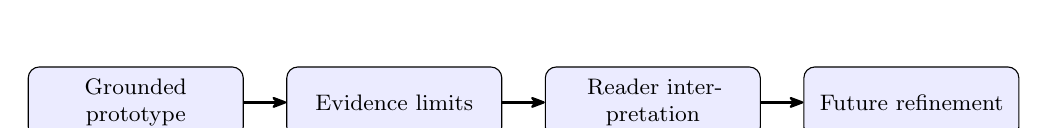
\begin{tikzpicture}[
  font=\small,
  scale=0.9,
  transform shape,
  box/.style={draw, rounded corners, align=center, text width=28mm, minimum height=10mm, fill=blue!8},
  arrow/.style={-{Stealth[round]}, thick}
]
\node[box] (a) {Grounded prototype};
\node[box, right=6mm of a] (b) {Evidence limits};
\node[box, right=6mm of b] (c) {Reader interpretation};
\node[box, right=6mm of c] (d) {Future refinement};

\draw[arrow] (a) -- (b);
\draw[arrow] (b) -- (c);
\draw[arrow] (c) -- (d);
\end{tikzpicture}
\caption{How the current limitations guide future refinement}
\label{fig:limitations_flow}
\end{figure}

\section{Chapter Conclusion }

The main limitations of AI-Scientist are its reliance on abstracts rather than full text, its lexical evidence
matching, its dependence on live-source coverage, and the case-study nature of its evaluation. These limitations do
not invalidate the central contribution, because the thesis is careful about what it claims: AI-Scientist is an
evidence-grounded, self-critical verification assistant that reports its uncertainty clearly and keeps its
conclusions aligned with the evidence it retrieves. The next chapter concludes the thesis and outlines future work
that follows directly from these limits.



\chapter[Conclusion]{Conclusion and Future Work}\label{chapter:conclusion}

\ChapterOpeningNote{This chapter summarizes the thesis findings, restates the main contributions, answers the
research questions, and outlines future work needed to move AI-Scientist toward deeper semantic verification and
broader, more reliable evidence coverage.}

\section{Conclusion }

This thesis presented AI-Scientist, a multi-agent orchestrated framework for scientific claim verification and
adaptive reasoning. The project began from a practical goal: given a research question, retrieve relevant
literature, extract its claims, verify each against evidence, inspect the weaker ones, and produce an
evidence-backed report with explicit confidence and a traceable record of the reasoning. The final contribution is
more specific and more defensible than simply ``an AI that answers research questions.'' AI-Scientist is a research
assistant that treats \emph{when to assert} and \emph{when to present a measured verdict} as first-class concerns.

The thesis deliberately avoids claiming to be the first system to ground answers in retrieved evidence, the first to
verify scientific claims against abstracts, or the first to use multiple cooperating agents. Prior work already
establishes each of these. AI-Scientist instead contributes a verification-first composition of these ideas, in
which the unit of output is a checked claim with a calibrated confidence and attributed evidence, realized as a
working system across arbitrary research domains \cite{lewis2020rag,thorne2018fever,wadden2020scifact,wu2023autogen}.

\section{Summary of Contributions }

The first contribution is the AI-Scientist architecture itself: a structured pipeline in which an Orchestrator
coordinates retrieval, claim extraction, verification, critique, synthesis, and reporting. The system grounds its
reasoning in a layered, source-prioritized evidence model and turns a research question into a set of verified
claims rather than a single undifferentiated paragraph, following the design direction of retrieval-grounded
systems and claim-level verification benchmarks \cite{guu2020realm,petroni2020kilt,thakur2021beir}.

The second contribution is a verification-first formulation of scientific question answering. By decomposing an
answer into atomic claims and attaching a verdict, an explicit confidence, and supporting evidence to each,
AI-Scientist makes factuality measurable at the level where support, contradiction, and uncertainty actually
differ \cite{honovich2022true,min2023factscore,es2023ragas}.

The third contribution is a transparent confidence and critique mechanism. Confidence is computed from evidence
strength, corroboration, and source independence and is bounded away from absolute certainty; a separate Critic
agent flags insufficient, low-confidence, single-source, and contradicted claims and drives a targeted, bounded
re-verification loop. Together these turn restraint and self-criticism from prompt instructions into engineered
system behaviour, consistent with recent self-refinement and multi-agent work \cite{shinn2023reflexion,yao2023treeofthoughts,asai2024selfrag}.

The fourth contribution is claim discipline. The thesis separates grounding from correctness, frames measured
responses as part of the system's design, and positions the multi-agent design against single-agent and RAG
baselines on a shared substrate so that its added value is isolated. That clarity is part of the scientific value
of the work: it makes clear where a grounded verifier helps and where it remains bounded by its evidence.
This kind of structured comparison is consistent with the spirit of established retrieval and factuality
evaluations \cite{lin2021truthfulqa,petroni2020kilt,ragsurvey2024}.

\section{Answers to the Research Questions }

RQ1 asked whether a multi-agent orchestrated framework improves verification quality and reasoning traceability
compared with a single-agent reader and a standard RAG pipeline. The evaluation supports this as the strongest
thesis claim: only the multi-agent system decomposes the answer into evidence-attributed claims, computes confidence
from corroboration and independence, handles contradiction, presents measured responses, and records a traceable
orchestration trace, whereas the baselines do none of these on the same evidence.

RQ2 asked whether grounding in a layered evidence base reduces unsupported claims. The system binds every supported
verdict to a retrieved sentence and returns insufficient evidence when no sentence aligns, which structurally
prevents the assertion of ungrounded claims; the layered model is confirmed to combine uploaded, curated, and live
evidence with the intended priority.

RQ3 asked whether per-claim confidence is a usable trust signal. The confidence behaves monotonically in evidence
strength, corroboration, and source independence, penalizes self-only corroboration, and never reaches certainty,
giving the user a transparent, well-behaved ordering of how trustworthy each conclusion is.

RQ4 asked whether an explicit critic-driven loop improves the handling of weak claims. The Critic reliably flags the
four weakness patterns and triggers targeted re-verification for the specific weak claims, concentrating additional
effort where the first pass is least settled.

RQ5 asked whether the system remains domain-general while rejecting non-research queries. The same workflow applies
across medicine, computer science, biology, and psychology, and the scope guard declines clearly non-research
queries with an explicit message, confirming both breadth and appropriate refusal.

\section{Future Work }

The most important future direction is deeper semantic verification. AI-Scientist currently matches evidence
primarily through token overlap and reasons over abstracts. Future systems should incorporate semantic entailment
models and full-text reading so that paraphrased support and subtle contradictions are detected, and so that
methodological details in the body of a paper inform the verdict. This direction aligns with broader advances in
retrieval-augmented and long-context reasoning systems \cite{karpukhin2020dpr,khattab2020colbert,guu2020realm}.

A second direction is stronger, learned confidence calibration. The current confidence is a transparent heuristic;
future work could calibrate it against labelled support judgments so that the reported number carries a frequentist
interpretation, while preserving the inspectability that makes the present design trustworthy. Work on calibrated
truthfulness and uncertainty-aware answering provides a natural starting point \cite{kadavath2022language,lin2021truthfulqa}.

A third direction is broader and more reliable evidence coverage. Connecting additional scholarly sources, handling
more document formats, and improving relevance ranking would extend the system's reach beyond the domains best
served by PubMed Central and arXiv, and would reduce its sensitivity to question phrasing.
A wider evidence base would also bring the system closer to benchmark settings used in large-scale retrieval
evaluation \cite{petroni2020kilt,thakur2021beir}.

A fourth direction is richer contradiction and consensus modelling. Beyond labelling a single claim as contradicted,
the system could characterize the state of a debate --- how many sources support each side and how strong each is
--- giving the user a map of the literature rather than a single verdict.
That would bring the system closer to the way scientific debates are discussed in fact-checking and literature
synthesis benchmarks \cite{thorne2018fever,wadden2020scifact,min2023factscore}.

A fifth direction is human-in-the-loop verification. Because AI-Scientist is designed to be inspectable, it is a
natural substrate for interactive workflows in which a researcher accepts, rejects, or refines individual claims and
the system updates its synthesis accordingly, combining machine recall with human judgement.
Such a workflow complements the broader trend toward cooperative, tool-using, and critique-aware language-model
systems \cite{wu2023autogen,asai2024selfrag}.

\begin{table}[!htbp]
\centering
\caption{Thesis-level takeaway and future direction}
\begin{tabularx}{0.94\linewidth}{>{\raggedright\arraybackslash}p{0.30\linewidth} >{\raggedright\arraybackslash}X}
\toprule
Area & Summary \\
\midrule
Core contribution & Verification-first scientific answering with traceable evidence \\
Observed strength & Measured confidence, contradiction handling, and critic-driven refinement \\
Current scope & Abstract-level, source-grounded evaluation across multiple domains \\
Future direction & Semantic reading, broader sources, and stronger calibration \\
\bottomrule
\end{tabularx}
\end{table}

\section{Final Remarks }

AI-Scientist does not solve scientific question answering, and the thesis does not need it to. The project shows
something more useful for the current state of language-model assistants: a research assistant must know when to
present a measured verdict. The evaluation demonstrates that grounding can be made visible, that confidence can be
made transparent, that contradiction can be surfaced, and that measured responses can be engineered rather than
hoped for. In response, AI-Scientist builds grounding, calibrated confidence, structured critique, and
traceability into the answering loop.

The final lesson is therefore practical as well as scientific. Future research assistants should not be judged only
by how fluently they answer. They should be judged by whether their conclusions are grounded, whether their
confidence reflects the evidence, and whether they surface disagreement. AI-Scientist is a step toward that kind
of assistant: a disciplined, evidence-aware collaborator whose reasoning a human can always inspect, consistent
with the broader direction of factuality-focused language-system research \cite{ji2023hallucination,huang2023hallucinationsurvey,es2023ragas}.




\appendix
\chapter{Reproducibility Artifacts}\label{appendix:artifacts}

\section{Purpose}

This appendix records the main components that support the AI-Scientist thesis. It is intended as a navigation aid
for examiners and future maintainers rather than as a replacement for the full project repository. The system is
implemented as a single Python package, \texttt{ai\_scientist}, with a Streamlit user interface and a FastAPI
service built on top of it.

\section{Core Modules}

\begin{table}[!htbp]
\centering
\caption{Core implementation modules of the AI-Scientist package.}
\label{tab:module-map}
\begin{tabular}{p{0.34\textwidth}p{0.55\textwidth}}
\toprule
Module & Responsibility \\
\midrule
\path{agents/orchestrator.py} & End-to-end workflow, early exits, and the re-verification loop. \\
\path{agents/retrieval.py} & Layered, source-prioritized retrieval and ranking. \\
\path{agents/live_retrieval.py} & Live retrieval from PubMed Central and arXiv. \\
\path{agents/claim_extraction.py} & Decomposition of abstracts into structured claims. \\
\path{agents/verification.py} & Evidence-bound verdicts and confidence computation. \\
\path{agents/critic.py} & Weakness critique and re-verification decisions. \\
\path{agents/synthesis.py} & Composition of the grounded executive summary. \\
\path{agents/report.py} & Structured and Markdown report assembly. \\
\path{models.py} & Typed dataclasses for papers, claims, evidence, and reports. \\
\path{config.py} & Settings: thresholds, source bonuses, and model configuration. \\
\path{utils.py} & Tokenization, Jaccard overlap, and query-coverage measures. \\
\path{scope.py} & Domain-general scope guard. \\
\path{llm.py} & Optional, provider-tolerant language-model refinement layer. \\
\path{corpus.py}, \path{ingestion.py} & Curated-corpus access and ingestion of user papers. \\
\path{baselines.py} & Single-agent and RAG comparison systems. \\
\bottomrule
\end{tabular}
\end{table}

\section{Interfaces}

\begin{table}[!htbp]
\centering
\caption{User-facing entry points.}
\label{tab:interface-map}
\begin{tabular}{p{0.30\textwidth}p{0.59\textwidth}}
\toprule
Entry point & Role \\
\midrule
\path{app.py} & Streamlit interface for uploading papers, selecting a model, asking questions, and inspecting per-claim verdicts, confidence, evidence, and the orchestration trace. \\
\path{ai_scientist/api.py} & FastAPI service exposing the same pipeline programmatically. \\
\bottomrule
\end{tabular}
\end{table}

\section{Verdict and Confidence Reference}

\begin{table}[!htbp]
\centering
\caption{Verdict space used by the Verification agent.}
\label{tab:verdict-map}
\begin{tabular}{p{0.26\textwidth}p{0.63\textwidth}}
\toprule
Verdict & Meaning \\
\midrule
\texttt{supported} & Retrieved evidence aligns with the claim; confidence scales with corroboration and source independence. \\
\texttt{contradicted} & Strong, multi-source counter-evidence dominates; the disagreement is reported explicitly. \\
\texttt{insufficient\_evidence} & No sufficiently aligned evidence, or the claim is overgeneralized; the system abstains. \\
\texttt{out\_of\_scope} & The query is not a research question and is declined before analysis. \\
\bottomrule
\end{tabular}
\end{table}

\section{Running the System}

The package is run with the source directory on the Python path. The deterministic pipeline operates fully offline
using the curated corpus and any uploaded papers; live retrieval from PubMed Central and arXiv is enabled through
the environment, optionally with an NCBI API key to raise the request rate; and the optional language-model
refinement is enabled when a provider API key is configured. Because the language model and live retrieval are
additive, the system produces the same structured assessment for a given question and evidence set whenever the
deterministic core alone is used.


\backmatter
\cleardoublepage
\addcontentsline{toc}{chapter}{References}
\begin{thebibliography}{99}
\bibitem{lewis2020rag}
Lewis, Patrick and Perez, Ethan and Piktus, Aleksandra and Petroni, Fabio and others. Retrieval-Augmented Generation for Knowledge-Intensive NLP. Advances in Neural Information Processing Systems (NeurIPS). 2020.

\bibitem{ragsurvey2024}
Gao, Yunfan and Xiong, Yun and Gao, Xinyu and others. Retrieval-Augmented Generation for Large Language Models: A Survey. arXiv:2312.10997. 2024.

\bibitem{ji2023hallucination}
Ji, Ziwei and Lee, Nayeon and Frieske, Rita and others. Survey of Hallucination in Natural Language Generation. ACM Computing Surveys. 2023.

\bibitem{huang2023hallucinationsurvey}
Huang, Lei and Yu, Weijiang and Ma, Weitao and others. A Survey on Hallucination in Large Language Models: Principles, Taxonomy, Challenges, and Open Questions. arXiv:2311.05232. 2023.

\bibitem{manakul2023selfcheckgpt}
Manakul, Potsawee and Liusie, Adian and Gales, Mark J. F.. SelfCheckGPT. Proceedings of the Conference on Empirical Methods in Natural Language Processing (EMNLP). 2023.

\bibitem{min2023factscore}
Min, Sewon and Krishna, Kalpesh and Lyu, Xinxi and others. FActScore. Proceedings of the Conference on Empirical Methods in Natural Language Processing (EMNLP). 2023.

\bibitem{wadden2020scifact}
Wadden, David and Lin, Shanchuan and Lo, Kyle and others. Fact or Fiction: Verifying Scientific Claims. Proceedings of the Conference on Empirical Methods in Natural Language Processing (EMNLP). 2020.

\bibitem{thorne2018fever}
Thorne, James and Vlachos, Andreas and Christodoulopoulos, Christos and Mittal, Arpit. FEVER. Proceedings of the Conference of the North American Chapter of the Association for Computational Linguistics (NAACL). 2018.

\bibitem{yao2023react}
Yao, Shunyu and Zhao, Jeffrey and Yu, Dian and others. ReAct. International Conference on Learning Representations (ICLR). 2023.

\bibitem{shinn2023reflexion}
Shinn, Noah and Cassano, Federico and Gopinath, Ashwin and Narasimhan, Karthik and Yao, Shunyu. Reflexion. Advances in Neural Information Processing Systems (NeurIPS). 2023.

\bibitem{asai2024selfrag}
Asai, Akari and Wu, Zeqiu and Wang, Yizhong and Sil, Avirup and Hajishirzi, Hannaneh. Self-RAG. International Conference on Learning Representations (ICLR). 2024.

\bibitem{dhuliawala2023cove}
Dhuliawala, Shehzaad and Komeili, Mojtaba and Xu, Jing and others. Chain-of-Verification Reduces Hallucination in Large Language Models. arXiv:2309.11495. 2023.

\bibitem{wu2023autogen}
Wu, Qingyun and Bansal, Gagan and Zhang, Jieyu and others. AutoGen. arXiv:2308.08155. 2023.

\bibitem{li2023camel}
Li, Guohao and Hammoud, Hasan Abed Al Kader and Itani, Hani and Khizbullin, Dmitrii and Ghanem, Bernard. CAMEL. Advances in Neural Information Processing Systems (NeurIPS). 2023.

\bibitem{du2023debate}
Du, Yilun and Li, Shuang and Torralba, Antonio and Tenenbaum, Joshua B. and Mordatch, Igor. Improving Factuality and Reasoning in Language Models through Multiagent Debate. arXiv:2305.14325. 2023.

\bibitem{es2023ragas}
Es, Shahul and James, Jithin and Espinosa-Anke, Luis and Schockaert, Steven. RAGAS. arXiv:2309.15217. 2023.

\bibitem{robertson2009bm25}
Robertson, Stephen and Zaragoza, Hugo. The Probabilistic Relevance Framework: BM25. Foundations and Trends in Information Retrieval. 2009.

\bibitem{ncbi_eutils}
National Center for Biotechnology Information. Entrez Programming Utilities (E-utilities. NCBI/NLM developer documentation. 2023.

\bibitem{arxiv_api}
arXiv. arXiv. Cornell University Library. 2023.

\bibitem{langgraph2024}
LangChain. LangGraph. Open-source framework documentation. 2024.

\bibitem{vaswani2017attention}
Vaswani, Ashish and Shazeer, Noam and Parmar, Niki and others. Attention Is All You Need. Advances in Neural Information Processing Systems (NeurIPS). 2017.

\bibitem{devlin2019bert}
Devlin, Jacob and Chang, Ming-Wei and Lee, Kenton and Toutanova, Kristina. BERT. Proceedings of the Conference of the North American Chapter of the Association for Computational Linguistics (NAACL). 2019.

\bibitem{raffel2020t5}
Raffel, Colin and Shazeer, Noam and Roberts, Adam and others. Exploring the Limits of Transfer Learning with a Unified Text-to-Text Transformer. JMLR. 2020.

\bibitem{petroni2019knowledgebases}
Petroni, Fabio and Rockta. Language Models as Knowledge Bases?. Proceedings of the Conference on Empirical Methods in Natural Language Processing (EMNLP). 2019.

\bibitem{guu2020realm}
Guu, Kelvin and Lee, Kenton and Tung, Zora and Pasupat, Panupong and Chang, Ming-Wei. REALM. Proceedings of the International Conference on Machine Learning (ICML). 2020.

\bibitem{karpukhin2020dpr}
Karpukhin, Vladimir and Ou g. Dense Passage Retrieval for Open-Domain Question Answering. Proceedings of the Conference on Empirical Methods in Natural Language Processing (EMNLP). 2020.

\bibitem{khattab2020colbert}
Khattab, Omar and Zaharia, Matei. ColBERT. Proceedings of the International Conference on Research and Development in Information Retrieval (SIGIR). 2020.

\bibitem{izacard2021fid}
Izacard, Gautier and Grave, Edouard. Leveraging Passage Retrieval with Generative Models for Open Domain Question Answering. Proceedings of the European Chapter of the Association for Computational Linguistics (EACL). 2021.

\bibitem{izacard2022atlas}
Izacard, Gautier and Lewis, Patrick and Lomeli, Maria and others. Atlas. Proceedings of the International Conference on Machine Learning (ICML). 2022.

\bibitem{thakur2021beir}
Thakur, Nandan and Reimers, Nils and Ru. BEIR. Proceedings of the Conference on Neural Information Processing Systems (NeurIPS). 2021.

\bibitem{rajpurkar2016squad}
Rajpurkar, Pranav and Zhang, Jian and Lopyrev, Konstantin and Liang, Percy. SQuAD. Proceedings of the Conference on Empirical Methods in Natural Language Processing (EMNLP). 2016.

\bibitem{joshi2017triviaqa}
Joshi, Mandar and Choi, Eunsol and Weld, Daniel and others. TriviaQA. Proceedings of the Association for Computational Linguistics (ACL). 2017.

\bibitem{yang2018hotpotqa}
Yang, Zhilin and Qi, Peng and Zhang, Saizheng and others. HotpotQA. Proceedings of the Conference on Empirical Methods in Natural Language Processing (EMNLP). 2018.

\bibitem{fan2020wikimultihopqa}
Ho, Xuan and others. 2WikiMultiHopQA. Proceedings of the Language Resources and Evaluation Conference (LREC). 2020.

\bibitem{chung2022truthfulqa}
Lin, Stephanie and Hilton, Jacob and Evans, Owain. TruthfulQA: Measuring How Models Mimic Human Falsehoods. Proceedings of the Annual Meeting of the Association for Computational Linguistics (ACL). 2022.

\bibitem{lin2021truthfulqa}
Lin, Stephanie and Hilton, Jacob and Evans, Owain. TruthfulQA: Measuring How Models Mimic Human Falsehoods. arXiv:2109.07958. 2021.

\bibitem{nakano2021webgpt}
Nakano, Reiichiro and Hilton, Jacob and Balaji, Sai and others. WebGPT. arXiv:2112.09332. 2021.

\bibitem{schick2023toolformer}
Schick, Timo and Dwivedi-Yu, Jane and Dess`i. Toolformer: Language Models Can Teach Themselves to Use Tools. Proceedings of the International Conference on Learning Representations (ICLR). 2023.

\bibitem{park2023generativeagents}
Park, Joon Sung and O'Brien, Joseph C. and Cai, Carrie J. and others. Generative Agents: Interactive Simulacra of Human Behavior. arXiv:2304.03442. 2023.

\bibitem{yao2023treeofthoughts}
Yao, Shunyu and Yu, Dian and Zhao, Jeffrey and others. Tree of Thoughts: Deliberate Problem Solving with Large Language Models. arXiv:2305.10601. 2023.

\bibitem{beltagy2019scibert}
Beltagy, Iz and Lo, Kyle and Cohan, Arman. SciBERT. Proceedings of the Conference on Empirical Methods in Natural Language Processing (EMNLP). 2019.

\bibitem{lee2019biobert}
Lee, Jinhyuk and Yoon, Wonjin and Kim, Sungdong and others. BioBERT. Bioinformatics. 2020.

\bibitem{gu2021pubmedbert}
Gu, Yuhao and Tinn, Robert and Cheng, Hao and others. Domain-Specific Language Model Pretraining for Biomedical Natural Language Processing. arXiv:2007.15779. 2021.

\bibitem{alsentzer2019clinicalbert}
Alsentzer, Emily and Murphy, John R. and Boag, William and others. Publicly Available Clinical BERT. Proceedings of the Clinical Natural Language Processing Workshop. 2019.

\bibitem{jin2019pubmedqa}
Jin, Qiao and Dhingra, Bhuwan and Liu, Zhengping and others. PubMedQA. Proceedings of the Conference on Empirical Methods in Natural Language Processing (EMNLP). 2019.

\bibitem{pal2022medmcqa}
Pal, Ankit and Umapathi, Logesh Kumar and Sankarasubbu, Malaikannan. MedMCQA. Proceedings of the Conference on Health, Inference, and Learning (CHIL). 2022.

\bibitem{jin2021medqa}
Jin, Di and Pan, Eileen and Oufattole, Nassim and others. What Disease Does This Patient Have? A Large-scale Open Domain Question Answering Dataset from Medical Exams. Applied Sciences 11(14):6421. 2021.

\bibitem{honovich2022true}
Honovich, Or and Aharoni, Roee and Herzig, Jonathan and others. TRUE. Proceedings of the Association for Computational Linguistics (ACL). 2022.

\bibitem{ouyang2022instructgpt}
Ouyang, Long and Wu, Jeffrey and Jiang, Xu and others. Training Language Models to Follow Instructions with Human Feedback. arXiv:2203.02155. 2022.

\bibitem{wei2022cot}
Wei, Jason and Wang, Xuezhi and Schuurmans, Dale and others. Chain-of-Thought Prompting Elicits Reasoning in Large Language Models. arXiv:2201.11903. 2022.

\bibitem{kojima2022zeroshotreasoners}
Kojima, Takeshi and Gu, Shixiang Shane and Reid, Maarten and others. Large Language Models are Zero-Shot Reasoners. arXiv:2205.11916. 2022.

\bibitem{wang2022selfconsistency}
Wang, Xuezhi and Wei, Jason and Schuurmans, Dale and others. Self-Consistency Improves Chain of Thought Reasoning in Language Models. arXiv:2203.11171. 2022.

\bibitem{borgeaud2022retro}
Borgeaud, Sebastian and Mensch, Arthur and Hoffmann, Jordan and others. Improving Language Models by Retrieving from Trillions of Tokens. Proceedings of the International Conference on Machine Learning (ICML). 2022.

\bibitem{zhou2022leasttomost}
Zhou, Denny and others. Least-to-Most Prompting Enables Complex Reasoning in Large Language Models. arXiv:2205.10625. 2022.

\bibitem{khandelwal2020knnlm}
Khandelwal, Urvashi and Lewis, Mike and Jurafsky, Dan and Zettlemoyer, Luke. Generalization through Memorization: Nearest Neighbor Language Models. arXiv:1911.00172. 2020.

\bibitem{lewis2020bart}
Lewis, Mike and Liu, Yinhan and Goyal, Naman and others. BART. arXiv:1910.13461. 2020.

\bibitem{petroni2020kilt}
Petroni, Fabio and Piktus, Aleksandra and Fan, Angela and others. KILT. arXiv:2009.02252. 2020.

\bibitem{kadavath2022language}
Kadavath, Saurav and Conerly, Tom and Askell, Amanda and others. Language Models (Mostly) Know What They Know. arXiv:2207.05221. 2022.

\bibitem{kuhn2023semantic}
Kuhn, Lorenz and Gal, Yarin and Farquhar, Sebastian. Semantic Uncertainty: Linguistic Invariances for Uncertainty Estimation in Natural Language Generation. arXiv:2302.09664. 2023.

\bibitem{wang2024self}
Wang, Yile and others. Self-Knowledge Guided Retrieval Augmentation for Large Language Models. arXiv:2310.05002. 2024.

\end{thebibliography}



\cleardoublepage
\FrontMatterChapter{Author's Biography}

\textbf{\ThesisAuthorName} is a postgraduate student of \textbf{\ThesisProgram} in the
\textbf{\ThesisDepartment}, \textbf{\ThesisInstitute}. Her academic journey has focused on developing a strong
foundation in computer science and on exploring research problems that combine intelligent systems, information
retrieval, and trustworthy reasoning. During her M.Tech studies, she has developed a particular interest in
multi-agent systems, retrieval-augmented generation, evidence-grounded reasoning, and the practical use of large
language models for scientific knowledge work.

She is presently working on the thesis project \emph{AI-Scientist: A Multi-Agent Orchestrated Framework for
Scientific Claim Verification and Adaptive Reasoning}. The project reflects her interest in building systems that
do not merely generate fluent responses, but instead organize evidence, verify claims, and present results in a
traceable and academically useful form. Through this work, she aims to contribute to the broader discussion on
reliable AI-assisted scientific analysis and evidence-aware question answering.

Beyond her academic pursuits, she values continuous learning, disciplined work, and thoughtful problem solving.
She is also interested in applying computational methods to real-world research workflows in ways that remain
transparent, dependable, and easy to interpret.
\clearpage

\cleardoublepage
\null
\clearpage

\end{document}
